\documentclass[sigconf]{acmart}

\usepackage{graphicx} \usepackage{balance} \usepackage{hyperref} \usepackage[all]{nowidow} \usepackage{float}
\usepackage{tikz} \usepackage{tikz-3dplot} \usepackage{nicefrac} \usepackage{algorithm} \usepackage{subcaption}
\usepackage[noend]{algpseudocode} \usepackage{array} \usepackage{pgfplots} \usepackage{booktabs} \usepackage{siunitx}
\usepackage{enumitem} \usepackage[utf8]{inputenc} \usepackage{amsmath} \usepackage{amssymb} \usepackage{filecontents}
\usepackage{amsfonts}

\newcommand{\vv}[1]{#1} % Not doing anything special for vectors right now...
\newcommand{\seq}{\!=\!}
\newcommand{\iFrame}{\mathcal{I}}
\newcommand{\kFrame}{\mathcal{K}}
\everypar{\looseness=-1}

\begin{document}
	\title{An Experimental Survey of Evaluation Strategies for Constellation Queries}

    \author{Glenn Galvizo}
    \email{glennga@hawaii.edu}
    \affiliation{%
        \institution{University of Hawaii at Manoa}
        \city{Honolulu}
        \state{Hawaii}
    }

    \author{Lipyeow Lim}
    \email{lipyeow@hawaii.edu}
    \affiliation{%
        \institution{University of Hawaii at Manoa}
        \city{Honolulu}
        \state{Hawaii}
    }

	%\begin{abstract}
%    The process of identifying stars is integral toward stellar based orientation determination in spacecraft.
%    Star identification involves matching points in an image of the sky with stars in an astronomical catalog.
%    A unified framework for identification was created and used to analyze six variations of methods based on their
%    approach to star set identification, obtaining a single image to catalog star set match, and uniquely mapping
%    each star in a image star set to a catalog star set.
%    Each method was presented an artificial image, and aspects that were interchangeable among each process were
%    normalized.
%    Given an image with false stars, the Pyramid method has the highest average accuracy and is the fastest of the six.
%    Given an image where each star's true position is distributed randomly (Gaussian noise), the Spherical Triangle
%    method's accuracy is the least sensitive.
%\end{abstract}

\begin{abstract}
    Given a set of query points within an image coordinate system, constellation queries identify the matching points in a database of known points within a standard coordinate system.
    Constellation queries are an integral part of orientation determination systems used in spacecrafts to orient and navigate themselves.
    The query points are bright spots in an image captured by a camera on the spacecraft and the database contains known celestial objects in a celestial coordinate system.
    This paper studies six existing constellation query processing strategies (Angle, Interior Angle, Spherical Triangle, Planar Triangle, Pyramid, Composite Pyramid) using a unified algorithmic framework and presents experimental evaluation of the six strategies.
    We find that the Pyramid strategy in its simplified form has the best accuracy to runtime ratio given simulated images with false positives, false negatives, and Gaussian noise.
\end{abstract}


	\copyrightyear{2019} 
	\acmYear{2019} 
	\setcopyright{acmcopyright}
	\acmConference[SSDBM '19]{31st International Conference on Scientific and Statistical Database Management}{July 23--25, 2019}{Santa Cruz, CA, USA}
	\acmBooktitle{31st International Conference on Scientific and Statistical Database Management (SSDBM '19), July 23--25, 2019, Santa Cruz, CA, USA}
	\acmPrice{15.00}
	\acmDOI{10.1145/3335783.3335806}
	\acmISBN{978-1-4503-6216-0/19/07}

	\begin{CCSXML}
		<ccs2012>
		<concept>
		<concept_id>10002951.10003317</concept_id>
		<concept_desc>Information systems~Information retrieval</concept_desc>
		<concept_significance>500</concept_significance>
		</concept>
		<concept>
		<concept_id>10002951.10003317.10003325</concept_id>
		<concept_desc>Information systems~Information retrieval query processing</concept_desc>
		<concept_significance>500</concept_significance>
		</concept>
		<concept>
		<concept_id>10002951.10003317.10003359.10003362</concept_id>
		<concept_desc>Information systems~Retrieval effectiveness</concept_desc>
		<concept_significance>500</concept_significance>
		</concept>
		<concept>
		<concept_id>10002951.10003317.10003359.10003363</concept_id>
		<concept_desc>Information systems~Retrieval efficiency</concept_desc>
		<concept_significance>500</concept_significance>
		</concept>
		</ccs2012>
	\end{CCSXML}

	\ccsdesc[500]{Information systems~Information retrieval}
	\ccsdesc[500]{Information systems~Information retrieval query processing}
	\ccsdesc[500]{Information systems~Retrieval effectiveness}
	\ccsdesc[500]{Information systems~Retrieval efficiency}

	\maketitle

    \keywords{
        information retrieval, performance analysis, query processing
    }

	\newcommand{\imageset}{\texttt{IMG}}
\newcommand{\databaseset}{\texttt{DB}}
\newcommand{\imagesubset}{b}
\newcommand{\databasesubset}{R}
\newcommand{\candidateset}{r}
\newcommand{\solutionmap}{h}

\newcommand{\genericdatabase}{\texttt{X\_DB}}
\newcommand{\angdatabase}{\texttt{ANG\_DB}}
\newcommand{\dotdatabase}{\texttt{DOT\_DB}}
\newcommand{\intdatabase}{\texttt{INT\_DB}}
\newcommand{\sphdatabase}{\texttt{SPH\_DB}}
\newcommand{\plndatabase}{\texttt{PLN\_DB}}
\newcommand{\pyrdatabase}{\texttt{PYR\_DB}}
\newcommand{\comdatabase}{\texttt{COM\_DB}}

\section{Introduction}\label{sec:introduction}
With the advent of commercial space industry, we are seeing an increasing number of spacecrafts, both manned and unmanned, launched into space.
One important function on a spacecraft is the ability to determine its orientation in space using the images captured by a camera on the spacecraft -- this is known as the \textit{Lost-in-space} problem.
For example, consider the design of low Earth orbit (LEO) spacecrafts.
In order for the spacecraft to point a payload, direct its thrusters, or orient its solar panels, an accurate \textit{attitude} (another term for orientation) must be known.
There are a few known landmarks in space where some attitude can be extracted (e.g.\ the Earth, the Sun), but most attitude determination systems instead use multiple stars within the field of view of a camera to determine their orientation.

The images capture a rectangular region of space -- think of an image of the sky at night from an Earth-centric perspective.
Each image is essentially a collection of bright spots (celestial objects) and their location in the image coordinate system.
To find the attitude of the spacecraft, we first have to match the pattern of celestial objects in the image to a database of known celestial objects.
We refer to such database queries as \textit{Constellation Queries}:
Given a set of query points in the image coordinate system, find the set of
points, i.e.\ constellations, in a database of known points (in a standard
coordinate system) that matches a subset of the query points.

Hypothetically, if we could transform the query points and database points to a
common coordinate system, then constellation queries would be a simple database
lookup for each query point. Unfortunately, evaluating constellation queries
are complicated by several issues. First the query points and the points in the
database are in two different coordinate systems and the transformation between
the two coordinate system is not known \emph{a priori}.
In fact, attitude determination \emph{is} finding the transformation between the two coordinate systems.
Second, the query points are affected by transient celestial objects (e.g.\ meteors) resulting in spurious points in the image, obstructions resulting in missing points, and camera characteristics resulting in deviations of the query point's true position.

%Ancient mariners could look up at the night sky, point out which stars they were looking at, and navigate across the
%globe without the use of maps.
%\textit{Star identification algorithms} refer to computational approaches to determining which stars are in the sky.
%Given an image of the sky, star identification is matching the bright spots in an image to stars in an astronomical
%catalog.
%The device that performs these computations is the star tracker, much like the navigators on the ship.
%\textit{Lost-in-space} refers to an additional constraint on the problem: the absence of knowing where we took
%the picture and how we pointed the camera.

%There exist roughly $4{,}500$ stars in the sky visible to the human eye.
%For an image of $n$ stars, the naive approach would be compute $C(4{,}500, n)$ combinations from this collection and
%compare each to some subset of stars found in the image.
%For $n\seq 3$, this requires over $10^{10}$ comparisons.
%As an alternative, we sacrifice storage and precision for speed by searching a separate collection which indexes the
%${\sim}4{,}500$ stars by one or more features.
%When this subset is identified, we determine and return the orientation of the image relative to collection
%of ${\sim}4{,}500$ stars.

%\subsection{Stellar Based Attitude Determination}\label{subsec:stellarBasedAttitudeDetermination}
%Attitude refers to the translation between how one system describes an object compared to how a different system
%describes the same object.
%
%In the context of spacecraft attitude for star identification, there exist three reference frames: the
%\textit{body frame}, the \textit{sensor frame}, and the \textit{inertial frame}.
%The body frame itself is fixed to the structure of the spacecraft, the sensor frame is fixed to the star tracker,
%and the inertial frame refers to some non-accelerating frame in which stellar objects are recorded.
%All observations from the spacecraft exist in the sensor frame, but can easily be rotated to align with the body frame
%(the sensor itself is fixed to the spacecraft chassis).
%Consequently, the body frame is used interchangeably with the sensor frame.
%To describe the craft itself, an inertial frame is required for finding a practical attitude.
%A star observed in the inertial frame is more predictable than the same star observed in a tumbling spacecraft, aiding
%the usage of the attitude with orientation dependent processes.
%Using all three, the goal of attitude determination becomes finding some method of translation between the inertial
%frame and the body frame.

%Let $\kFrame$ describe an inertial coordinate system for $\databaseset$, our reference objects, and $\iFrame$ describe a body coordinate system for $\imageset$, the set of objects in the query image.
%For simplicity, we make the assumption here that all stars in $\kFrame$ are fixed and exist in an inertial frame known as the \textit{Earth centered inertial} (ECI) frame.
%The star vectors themselves come from astronomical catalogs, recorded as points lying on the celestial sphere~\cite{tappe:starTrackerDevelopment}.
%Two pieces of information are given here: right ascension $\alpha$ (equivalent to latitude on Earth) and declination $\delta$ (equivalent to longitude).
%The vector $\vv{\databaseset[j]}$ represents a point $\left( \alpha, \delta \right)$ lying on the surface of a sphere with constant radius, in 3D Cartesian space.
%Let $\vv{\imageset[j]}$ represent a 3D point projected from a 2D observation taken by the star tracker.
%A basic star tracker is composed of a camera, a computer for determining orientation, and a link back to the main computer.
%After taking the picture, the pixel positions of potential stars in the image are determined.
%This involves finding bright blobs in the image, and computing each blob's center of mass to get a point ($x, y$).
%Through some projection process involving the camera's lens structure (e.g.\ the inverse Mercator projection~\cite{weisstein:mercator}), $\vv{\imageset[j]}$ is then obtained~\cite{tappe:starTrackerDevelopment}.

%Let the matrix $A$ represent the transformation from $\kFrame$ to $\iFrame$.
%In 1965, Grace Wahba first formulated the attitude determination
%problem as finding an $A$ that minimizes the loss function~\cite{wahba:attitudeEstimationProblem}:
%\begin{equation}
%    L(A) = \frac{1}{2} \sum_j^n \vv{w_j} \left\| \vv{\imageset[j]} - A \times \vv{\databaseset[j]} \right\|^2
%\end{equation}
%where $\vv{w_j}$ represents a nonnegative weight associated with the noise between the query points $\vv{\imageset[j]}$ in the body frame and the matching points $\vv{\databaseset[j]}$ in the inertial frame.
%The \textit{TRIAD method} (short for TRIaxial Attitude Determination) is typically used as a closed form solution~\cite{markley:attitudeDeterminationTwoVectors} to Wahba's problem after evaluating the constellation query to retrieve the matching set of points from the database.
%Hence, constellation queries do not deal with finding the transformation matrix $A$, but focus on finding the sets of points, i.e.\ constellations, in a database of known points (in a standard coordinate system) that best matches a set of query points (in the image coordinate system) in the query image.

The constellation queries studied in this paper can be viewed as a type of
\emph{subgraph isomorphism query} that aims to find some 1-to-1 mapping between
the vertices in two graphs (i.e.\ the reference database and the image) if it
exists~\cite{scott:graphIsomorphismProblem}. The subgraph isomorphism
formulation is often juxtaposed with \emph{pattern recognition approaches},
which map larger sets of points within a defined field-of-view across some
reference table and image~\cite{padgett:gridAlgorithm}.
We also focus on \emph{non-recursive} constellation queries -  
queries that does not process results from an \emph{prior} query.
In recursive searches such as the SP-Search and SNA by
Samaan~\cite{samaan:recursiveMode}, an additional filter can be applied to the
query that limits the possible database points that map to our image set.
We are also interested in indexing strategies for constellation queries.
we indexed our reference relations solely by some statistic of a collection of
star positions (e.g.\ the interstar angle between two points, the area between
three points), rather than indexing by star brightnesses (see Scholl\cite{scholl:starFieldIdentification}, Ketchum~\cite{ketchum:onboardStarIdentification}, and more recently Zhang et. al~\cite{zhang:brightnessReferenced}).
There is also much prior work on optimizing the data accesses in
constellation queries, most notably Motari's SLA (Search-Less
Algorithm)~\cite{mortari:kVectorApproach}. Our focus is on the end-to-end
constellation query and not just on the data access aspects. 

This paper is an empirical survey of six existing constellation query processing strategies in the literature and in the industry.
%The six strategies are: the Angle strategy, the Interior Angle strategy, the Spherical Triangle strategy, the Planar Triangle strategy, the Pyramid strategy, and the Composite Pyramid strategy.
%Our contributions are as follows:
%\begin{itemize}
%    \item Development of a unified framework for describing six existing constellation query processing strategies.
%    \item Implementation of all six existing constellation query processing algorithms / strategies.
%    \item Extensive empirical evaluation of the six constellation query processing algorithms using the Hipparcos database and synthetic query images.
%\end{itemize}
To the best of our knowledge, no systematic survey exists for these constellation query processing algorithms, no attempts have been made to study them in a unified framework, and no empirical evaluation of these algorithms have been done even though many of these algorithms have been deployed in spacecrafts and satellites (SAS-3, HTSE, ISC~\cite{gottlieb:spacecraftAttitudeDetermination,mortari:pyramidIdentification}).
Additional survey papers have been published by Spratling~\cite{spratling:surveyStarIdentification} and
Br\"{a}tt~\cite{bratt:analysisStarIdentification}, but our research focuses on the specific area of constellation
queries (not image processing, attitude determination, or database searching) and describes each strategy within a unified framework.

%Our analysis focuses on a hardware-independent comparison of constellation query processing strategies and does not
%address the preprocessing of an image to identifying blobs.

%For $n \!>\! 2$, Wahba's problem exists as an optimization problem.
%In the $n\seq2$ case though, the \textit{TRIAD method} (short for TRIaxial Attitude Determination) exists as a
%closed form solution~\cite{markley:attitudeDeterminationTwoVectors}.
%This algorithm starts by constructing two sets of basis vectors: one attached to the body referential (two
%observations in the body frame) $\left[ \vv{t_{1I}} \ \vv{t_{2I}} \ \vv{t_{3I}} \right]$ and another attached to
%the inertial referential (two observations in the inertial frame) $\left[ \vv{t_{2I}} \ \vv{t_{2K}} \ \vv{t_{3K}}
%\right]$~\cite{benet:swisscubeAttitudeDetermination,black:passiveAttitudeDetermination}.
%This is known as the triad frame:
%\begin{alignat}{4}
%    \vv{t_{1I}} &= \frac{\vv{v_1}}{\left| \vv{v_1} \right|} &\vv{t_{2I}} &{}={}&
%    \frac{\vv{u_1}}{\left| \vv{u_1} \right|} \ \ \ \ \ \ \  \\
%    \vv{t_{2I}} &= \frac{\vv{v_1} \times \vv{v_2}}{\left| \vv{v_1} \times \vv{v_2} \right|} \ \ \ \ \ \ \ \
%        &\vv{t_{2K}} &{}={}& \frac{\vv{u_1} \times \vv{u_2}}{\left| \vv{u_1} \times \vv{u_2} \right|} \\
%    \vv{t_{3I}} &= \vv{t_{1I}} \times \vv{t_{2I}} &\vv{t_{3K}} &{}={}& \vv{t_{2I}} \times \vv{t_{2K}}
%\end{alignat}
%Getting from frame $\kFrame$ to $\iFrame$ now simplifies to multiplication of the triad frame base change matrices:
%\begin{equation}
%    A =
%    \begin{bmatrix}
%        \vv{t_{1K}} & \vv{t_{2K}} & \vv{t_{3K}}
%    \end{bmatrix}
%    \begin{bmatrix}
%        \vv{t_{1I}} & \vv{t_{2I}} & \vv{t_{3I}}
%    \end{bmatrix}^T
%\end{equation}

%\begin{subequations}
%Relative to our solar system, the majority of bright stars ($m \!<\! 6.0$, or visible from the Earth with the naked
%eye) do not visibly move.
%Relative to our solar system, the majority of stars visible from Earth with the naked eye do not visibly move.
%    To align these stars with the ones in the catalog, the inverse Mercator mapping is used [CITE ME]:
%    \begin{align}
%        x &= k \cos\left( \frac{x}{R}  \right) \cos\left(2 * \arctan\left(\exp\left(\frac{y}{R}\right)\right) -
%            \frac{\pi}{2}\right) \\
%        y &= k \cos\left( \frac{x}{R}  \right) \sin\left(2 * \arctan\left(\exp\left(\frac{y}{R}\right)\right) -
%            \frac{\pi}{2}\right) \\
%        z &= k \sin\left( \frac{x}{R}  \right)
%    \end{align}

%The rest of the paper is organized as follows:
%Related work is presented in the next section.
%Section~\ref{sec:starIdentificationMethods} describes the different constellation query processing strategies using
%our unified framework.
%Section~\ref{sec:empiricalEvaluation} presents our experimental evaluation of the different strategies.
%Section~\ref{sec:conclusion} draws conclusions.

	\newcommand{\nsubparagraph}[1]{\paragraph{#1:}}

%\section{Related Work}\label{sec:relatedWork}
\begin{figure}
    \centering{
    \usetikzlibrary{shapes.geometric, arrows}

% Style for process block.
\tikzstyle{process} = [rectangle, text width=2.5cm, minimum width=2.5cm, minimum height=1.5cm,text centered, draw=black,
fill=orange!30]

% Style for terminal block.
\tikzstyle{terminal} = [rectangle, text width=2cm, minimum width=2cm, minimum height=1.5cm,text centered,
draw=black, fill=red!30]

% Style for decision block.
\tikzstyle{decision} = [diamond, text width=1.5cm, minimum width=2.5cm, minimum height=2.5cm,text centered, draw=black,
fill=green!30, inner sep=-12pt]

% Style for line.
\tikzstyle{line} = [draw, -latex']

\begin{tikzpicture}[node distance=1.3cm, scale=0.77, transform shape]
    \node[scale=1](getImage)[terminal]{Given Image Set, Reference Database};
    \node[scale=1](pickQueryStars) [process, left of=getImage, xshift =-2.2cm] {Select Subset from Image Set};
    \node[scale=1](searchCatalog)[process, below of=pickQueryStars, yshift=-0.7cm] {Query Reference with Feature Predicate(s)};
    \node[scale=1](confidentInCatalog)[decision, below of=searchCatalog, yshift=-1cm] {Query Yields Sole Result?};
%    \node[scale=1](filterCandidates)[process, below of=confidentInCatalog, yshift=-0.4cm] {Select Candidate $R[1]$};
%    \node[scale=1](confidentAfterFilter)[decision, below of=filterCandidates, yshift=-0.4cm] {Confident?};
    \node[scale=1](findMap)[process, below of=confidentInCatalog, yshift=-1.2cm]{Map Image and Reference Subsets Together};
    \node[scale=1](confidentInMap)[decision, below of=findMap, yshift=-1cm] {Confident in Map?};
    \node[scale=1](returnMap)[terminal, right of=confidentInMap, xshift = 2.2cm] {Return Mapping, Image Subset};

    \draw[->,>=stealth](getImage.west) -- (pickQueryStars.east);
    \draw[->,>=stealth] (pickQueryStars) -- (searchCatalog);
    \draw[->, >=stealth] (searchCatalog) -- (confidentInCatalog);
    \draw[->,>=stealth] (confidentInCatalog) -- node[anchor=east, yshift=0.1cm]{Yes}(findMap);
%    \draw[->, >=stealth] (confidentInCatalog) -- node[anchor=east, yshift=0.1cm]{Yes}(filterCandidates);
%    \draw[->, >=stealth] (filterCandidates) -- (findMap);
%    \draw[->, >=stealth] (confidentAfterFilter) -- node[anchor=east, yshift=0.1cm]{Yes} (findMap);
    \draw[->, >=stealth] (findMap) -- (confidentInMap);
    \draw[->, >=stealth] (confidentInMap) -- node[xshift=0cm, yshift=0.25cm]{Yes} (returnMap);

    \draw[->, >=stealth] (confidentInCatalog.west) -- ++(-1.4cm, 0cm) node[anchor=south, xshift=0.5cm]{No}
    |- (pickQueryStars.west);
%    \draw[->, >=stealth] (confidentAfterFilter.west) -- ++(-1.4cm, 0cm) node[anchor=south, xshift=0.5cm]{No}
%    |- (pickQueryStars.west);
    \draw[->, >=stealth] (confidentInMap.west) -- ++(-1.4cm, 0cm) node[anchor=south, xshift=0.5cm]{No}
    |- (pickQueryStars.west);
\end{tikzpicture}
    \caption{
    Flowchart depicting the unified identification framework which all strategies here follow.
    Given a query image, this process returns a map that pairs of subset of these image stars with points in a reference database.
%    Given a query set $\imageset$, this process returns a function $\solutionmap$ whose domain is some subset of the image $\imagesubset$ and whose codomain is the stellar database, $\databaseset$.
%    In the event all subsets are exhausted, an error is raised and no map is returned (not depicted).
    } \label{figure:unifiedIdentificationFlowchart}
    }
\end{figure}



%This section serves to give a brief overview of the different approaches to querying for constellations.

%
%\nsubparagraph{Identification Classes}
%The first main class of identification and the focus of this paper is the \textit{subgraph isomorphism} class.
%Subgraph isomorphism is a NP complete problem which aims to find some 1-to-1 mapping between the vertices (points) in two graphs (i.e.\ the database and the image) if it exists~\cite{scott:graphIsomorphismProblem}.
%This involves describing and mapping sets of points between both the database and image in terms of various features relative to each other.
%
%The second class of identification is the \textit{pattern recognition} class.
%In contrast to subgraph isomorphism class, the pattern recognition class commonly deals with larger sets of points within some defined field-of-view and matches patterns rather than features.
%Pattern formation typically involves 2D binary matrices (grids), where `1' occupies a cell with a point and `0' occupies a cell without one~\cite{padgett:gridAlgorithm}.

%
%
%Another notable attempt toward pattern formation utlizes Delaunay Triangulation, as seen from Miri~\cite
%
%Some notable approaches utilize Padgett's~\cite{padgett:gridAlgorithm} and Lee's~\cite{lee:modifiedGridAlgorithm}
%use of binary matrices (grids) to construct patterns, Lindsey~\cite{lindsey:neuralNetworkMethods} and
%Alvelda's~\cite{alvelda:neuralNetworkStar} use of neural networks to optimize pattern similarity, and
%Paladugu's~\cite{paladugu:geneticAlgorithms} use of a genetic algorithm to solve the same pattern similarity problem.

%\nsubparagraph{Recursive Property}
%Recall that the lost-in-space condition specifies that we do not have any information about the spacecraft's attitude prior to starting our query.
%For the majority of a star tracker's operation though, this constraint can be relaxed to allow for the use of \textit{recursive} constellation querying.
%Recursive strategies possess an attitude recorded at time $t$, and perform another query at a later time $t + dt$.
%Two strategies proposed by Samaan (SP-Search and SNA) reduce the amount of candidate points from the database that could map to query points from the image~\cite{samaan:recursiveMode}.

%\nsubparagraph{Features}
%Each point has a position associated with it, be it from a star database or from the image.
%Using this position, the most common feature is the interstar angle between two points, first utilized by Gottlieb to identify sets of three points with three interstar angles~\cite{gottlieb:spacecraftAttitudeDetermination}.
%Notable strategies with geometric functions utilizing these angles were proposed by: Groth~\cite{groth:patternMatchingMethod}, Cole \& Crassidus~\cite{coleAndCrassidis:sphericalTriangleMethod,coleAndCrassidis:planarTriangleMethod}, and Lang~\cite{lang:astrometryDotNet}.
%Another common feature is the interior angle between three points, where one point exists as a vertex to two other points.
%Liebe uses this in conjunction with interstar angles~\cite{liebe:starTrackersAttitudeDetermination}.

%Each star has a position associated with it, be it from a star catalog or from the image.
%Using this position, the most common feature is the interstar angle between two stars, first utilized by Gottlieb to
%identify sets of three stars with three angles~\cite{gottlieb:spacecraftAttitudeDetermination}.
%Additional geometric functions utilizing these interstar angles were proposed by: Groth (using the log of the sum of
%three interstar angles in a trio~\cite{groth:patternMatchingMethod}), Cole \& Crassidus (treating the angles of a
%star trio as sides to a triangle, and computing the triangle's area and
%torque)~\cite{coleAndCrassidis:sphericalTriangleMethod, coleAndCrassidis:planarTriangleMethod}, and Lang (using the
%differences in interstar angle between a star quad in a localized coordinate system)~\cite{lang:astrometryDotNet}.
%Another common feature is the interior angle between three stars, where one star exists as a vertex to two other stars.
%Liebe uses this in conjuction with interstar angles~\cite{liebe:starTrackersAttitudeDetermination}.

%This feature is used solely by Rousseau (the sine of the closest two closest stars of a trio)
%~\cite{rousseau:starRecognitionAPS}
%and Samaan (the interior angles of three stars)
%~\cite{samaan:nondimensionalStarIdentification},
%and in conjunction with the interstar angles by Liebe~\cite{liebe:starTrackersAttitudeDetermination}.

%Each point also has a brightness attached it, a feature less commonly used due to large variance in measurement.
%Spratling describes two early strategies to take advantage of this feature.
%Scholl proposed the usage of this to remove the need for ambiguity after matching subsets with angular features ~\cite{scholl:starFieldIdentification}.
%Ketchum later introduced the second sequential filtering algorithm, which identifies two points using their brightness in comparison to the common trio required of angle strategies~\cite{ketchum:onboardStarIdentification}.
%More recent work toward integrating brightness more heavily has been performed by Zhang et. al~\cite{zhang:brightnessReferenced}.
%
%\nsubparagraph{Database Access}
%The naive approach to searching for matching features in a subgraph isomorphism approach is to perform a linear search across an entire set in a database and search for matching subsets.
%%Early star identification strategies focused on reducing the size of the relation to be searched, rather than the search
%%process itself.
%In 1996, Quine (according to Spratling) was the first to reduce the database search time from linear to log time using a binary search tree~\cite{quine:fastAutonomousStarAcquistion}.
%The following year Mortari's "Search-Less Algorithm" was introduced, which utilizes $k$-vectors to retrieve multiple nearby stars at once, rather than one at a time~\cite{mortari:kVectorApproach}.

\newcommand{\srightarrow}{\! \rightarrow \!}
%\nsubparagraph{Mapping}
%Identification is a process that pairs point(s) in an image to star(s) in a database.
%Gottlieb's strategy used a voting approach to remove the ambiguity after identifying a single point pair~\cite{gottlieb:spacecraftAttitudeDetermination}, which was later generalized by Kolomenkin to vote for every point in the image~\cite{kolomenkin:geometricVoting}.
%The direct match test was proposed by Needleman (according to Tappe), which determines the likelihood of a map based on how many points from each frame align with the attitude formed by the map~\cite{needelman:stellarAttitudeAcquisition}.
%In an effort to avoid the mapping processes above, Anderson (according to Spratling) proposed the use of storing permutations of point subsets instead of combinations at the expense of storage~\cite{anderson:autonomousStarSensing}.
%The use of neural networks~\cite{lindsey:neuralNetworkMethods,alvelda:neuralNetworkStar} and genetic algorithms~\cite{paladugu:geneticAlgorithms} have also been proposed to optimize the mapping process.

	\newcommand{\algorithmautorefname}{Algorithm}

\newcommand{\algeqref}[1]{\hyperref[#1]{Eq.~\ref*{#1}}}
\algnewcommand{\LineComment}[1]{\State \(\triangleright\) #1}
\algrenewcommand\algorithmicindent{0.35cm}
\newcommand{\bigO}{\mathcal{O}}
\newcommand{\abs}[1]{\left| #1 \right|}
\newcommand{\set}[1]{\left\{ #1 \right\}}
\MakeRobust{\Call}

\newfloat{algorithm}{t}{lop}
\restylefloat{algorithm}

\section{Constellation Query Processing Strategies}\label{sec:starIdentificationMethods}
This section serves to describe our unified framework and a high-level overview of how six different approaches both adhere to this framework \& how they differ from each other.
%Six different approaches to constellation query processing are described in this section.
%When the description did not specify a step in this flow, a simple or existing approach from another strategy was used.
%Several deviations to the algorithms from the original literature were introduced from newer literature to evaluate
%the effectiveness of these changes.

\subsection{Unified Identification Strategy Framework}\label{subsec:unifiedIdentification}
Each constellation query is presented with a set of points from an image $\imageset$ of size $n$ as well as a database containing two relations: one holds the collection of all known points $\texttt{REF}$ indexed by some identifier, and the other holds sets of these known points indexed by one or more features of the set itself: $R$.
Elements in $R$ are henceforth referred to as $r$ sets, with $\abs{r}\seq d$. 
The resultant is an $d$-sized subset of points from the image known as the $b$ set, as well as an injection from this subset to the database.
Identification of all points in each image is not the focus.

To start, all strategies begin by choosing a $b$ set from the image $\imageset$.
$r$ sets are then retrieved from $R$ using some predicate dependent on the current $b$.
If there exists only one $r$ as a result, then we proceed.
Otherwise, we loop back to the first step and select a different subset of $d$ stars.
Certain methods may also choose to invoke a secondary database retrieval utilizing a new database set to filter the current $r$ before deciding to choose a different $b$ altogether.
Once we have found a unique $r$ set, we determine a mapping between this set and $b$.
If we are confident in this map, we return this function along with the current $b$ set.
Otherwise, we loop back to the start and choose another $b$ set.
This process is depicted in~\autoref{figure:unifiedIdentificationFlowchart}.
In the event we exhaust all possible $b$ sets, an error is raised and no map is returned.

%Every algorithm starts with some combination from all possible $d$ combinations of $n$ points, where $d$ is the size of the image subset specified by the specific identification strategy.
%The image subset $\imagesubset$ is selected using one of these combinations.
%For a strategy that uses $d\seq2$ points to determine the mapping in an image of $n\seq 4$ points, the 6 combinations of $\imageset$ are given as $\binom{\imageset}{d}$:
%\begin{equation}
%    \begin{aligned}
%	    \binom{\imageset}{d} = \{&
%	    	\set{\vv{\imageset[1]}, \vv{\imageset[2]}},
%	    	\set{\vv{\imageset[1]}, \vv{\imageset[3]}}, \\
%	       &\set{\vv{\imageset[1]}, \vv{\imageset[4]}}, \ldots,
%	        \set{\vv{\imageset[3]}, \vv{\imageset[4]}}
%	        \}
%    \end{aligned}
%\end{equation}

%Each identification method $\texttt{X}$ is also presented a set $\genericdatabase$, composed of $d$ sized sets of all possible combinations or permutations of points from $\databaseset$.
%Using certain features of the image subset, the entire $\genericdatabase$ set is filtered to a set of star sets $\databasesubset$.
%This is known as the \emph{candidate retrieval step}.
%Referencing the same $d\seq 2$ strategy as before, an image subset $\imagesubset \seq \set{\vv{\imageset[1]}, \vv{\imageset[2]}}$ may yield the candidates in~\autoref{eq:catalogCandidateExample}:
%\begin{equation}
%	\label{eq:catalogCandidateExample}
%    \databasesubset = \set{ \set{\vv{\databaseset[104]}, \vv{\databaseset[899]}}, \set{\vv{\databaseset[7622]}, \vv{\databaseset[7771]}}, \ldots) } 
%\end{equation}

%Through some filter process for $\databasesubset$ and/or loop back to the $b$ selection step until $\abs{R} = 1$, a single set $\candidateset$ from the database candidates is  chosen.
%This is known as the \emph{candidate selection step}.
%The candidate selected here refers to a database star set that is likely to align with the current image subset.
%For a process that only loops back to the $b$ selection step until the $|\databasesubset| \seq 1$ criterion holds true, the following sequence of events may occur.
%The notation $\databasesubset^{(t)}$ and $\imagesubset^{(t)}$ denotes distinct $\genericdatabase$ and $\imageset$ subsets here, as opposed to the notation $\databasesubset[j]$ and $\imagesubset[j]$ which denotes singular database candidates and single points in $\imageset$ respectively.
%\begin{description}[noitemsep]
%    \item[$t = 1:$] $\text{ query with } b^{(1)}, \text{ get } R^{(1)} = \{\vv{r_{11}}, \vv{r_{12}}, \ldots\}.$
%    \item[$t = 2:$] $\abs{ R^{(1)} } \neq 1, \text{ criterion not met. }$
%    \item[$t = 3:$] $\text{ choose new image subset } b^{(2)}.$
%    \item[$t = 4:$] $\text{ query with } b^{(2)}, \text{ get } R^{(2)} = \{\vv{r_{21}}\}.$
%    \item[$t = 5:$] $\abs{ R^{(2)} } = 1, \text{ criterion met. }$
%    \item[$t = 6:$] $\text{ return } r, r \in R^{(2)} (\text{sole element in } R^{(2)} ).$
%\end{description}
%\begin{align*}
%    &t = 1, \text{ retrieve with } \imagesubset^{(1)}, \text{ get } \databasesubset^{(1)} = \{\vv{\candidateset_{11}}, \vv{\candidateset_{12}}, \ldots\}. \\
%    &t = 2, \ \abs{ \databasesubset^{(1)} } \neq 1, \text{ criterion not met. } \\
%    &t = 3, \text{ choose new image subset } \imagesubset^{(2)}. \\
%    &t = 4, \text{ retrieve with } \imagesubset^{(2)}, \text{ get } \databasesubset^{(2)} = \{\vv{\candidateset_{21}}\}. \\
%    &t = 5, \ \abs{ \databasesubset^{(2)} } = 1, \text{ criterion met. } \\
%    &t = 6, \text{ return } \candidateset, \candidateset \in \databasesubset^{(2)} (\text{sole element in } \databasesubset^{(2)} ).
%\end{align*}

%\begin{algorithm}
%	\caption{Direct Match Testing} \label{algorithm:dmt}
%	\begin{algorithmic}[1]
%		\Function{FPO}{$\texttt{DB\_NEAR}$, $\imageset$, $A$}
%		\State $\texttt{IMG\_ROT} \gets$ points in $\imageset$ rotated by $A$
%		\State \textbf{return} \parbox[t]{0.8\linewidth}{\raggedright all points in $\texttt{DB\_NEAR}$ that overlap with some point in $\texttt{IMG\_ROT}$}
%		\EndFunction
%		\\
%        \Function{DMT}{$b, r, \imageset, \databaseset$}
%        \State $\texttt{DB\_NEAR} \gets $ all points in $\databaseset$ near $r$
%        \State $\texttt{DB\_MATCH} \gets \emptyset$
%        \For {$h \in $ all possible mappings between $b$ and $r$}
%        \State $A \gets $ \Call{TRIAD}{$h, \imagesubset, \candidateset$}
%        \State $\texttt{DB\_MATCH}_h \gets $ \Call{FPO}{$\texttt{DB\_NEAR}, \imageset, A$}
%        \EndFor
%        \If{there exists no largest set $\texttt{DB\_MATCH}_h \in \texttt{DB\_MATCH}$}
%        \State \textbf{return} an invalid function %\Comment Indicate non-confidence.
%        \Else
%        \State \textbf{return} $h \in H$ associated with largest set in $\texttt{DB\_MATCH}$
%        \EndIf
%        \EndFunction
%	\end{algorithmic}
%\end{algorithm}

\newcommand{\smapsto}{\! \mapsto \!}
%\begin{subequations}
%	From here, a mapping $\solutionmap$ is determined that pairs each point found in the image subset to a single point in the database candidate set.
%	For brevity, it is assumed that all functions in this paper have domain $\imagesubset$ and codomain $\databaseset$.
%	Most (but not all) of the following queries utilize Tappe's implementation of the strategy and perform a \textit{direct match test}, abbreviated henceforth as DMT~\cite{tappe:starTrackerDevelopment,needelman:stellarAttitudeAcquisition}.
%    Given an image pair $\imagesubset$ and a database pair $\candidateset$, the following is proposed:
%    \begin{equation}
%        \solutionmap_1 \mid \solutionmap_1(\imagesubset[1]) = \candidateset[1], \ \solutionmap_1(\imagesubset[2]) = \candidateset[2]
%    \end{equation}
%    Wahba's problem is then solved using the TRIAD method to obtain a rotation $A_1$ between the image and database coordinate systems.
%    The \Call{TRIAD}{} function accepts a mapping $\solutionmap$, an image subset $\imagesubset$, a candidate set $\candidateset$, and outputs a rotation matrix $A$.
%    This process is repeated for the other possible permutation to obtain a second rotation $A_2$:
%    \begin{equation}
%        \solutionmap_2 \mid \solutionmap_2(\imagesubset[1]) = \candidateset[2], \ \solutionmap_2(\imagesubset[2]) = \candidateset[1]
%    \end{equation}
%\end{subequations}
%The most likely attitude is determined by the \Call{FPO}{} (short for \textit{Find Positive Overlay}) method, which returns how many points from $\imageset$ align with $\databaseset$ given rotation $A_1$ or $A_2$.
%The mapping with the most aligned points is then returned, and our query is completed.
%If there exists no singular mapping which gives us a largest set, we signal our lack of confidence to our caller by returning an invalid function.
%This process is detailed in~\autoref{algorithm:dmt}.
%
%If we are not confident in $h$ at this stage, another image subset is chosen and the process is repeated.
%This entire flow is detailed in~\autoref{figure:unifiedIdentificationFlowchart}.
%In the event $\binom{\imageset}{d}$ has been exhausted, an error is raised and no map is returned.

% Leaving this out for now. The flowchart should explain the process better.
%\begin{algorithm}[ht] \setstretch{1.0}[H]
%    \caption{Generic Star Identification Method} \label{algorithm:genericStarIdentification}
%    \begin{algorithmic}[1]
%        \Procedure{Identify}{}
%        \State $I \gets $ all stars from image
%        \For{$c \in r_k^{|I|}$}
%        \State $b \gets \{I(c_1), I(c_2), I(c_3), \dots, I(r_k)\}$
%        \State $R \gets $ catalog star sets, each set of size $=k$
%        \State $r \gets $ a single set from $R$ that matches $b$
%        \State $a \gets $ a map between $b$ and $r$
%        \\
%        \If{the steps above are successful}
%        \State \textbf{return} $a$
%        \EndIf
%        \EndFor
%        \EndProcedure
%    \end{algorithmic}
%\end{algorithm}

% Citation: https://digitalcommons.usu.edu/cgi/viewcontent.cgi?article=2723&context=etd AND Gottlieb.
\subsection{Overview of Strategies}\label{subsec:strat}
We discuss six strategies in this section: the Angle strategy (ANG), the Interior Angle strategy (INT), the Spherical Triangle strategy (SPH), the Planar Triangle strategy (PLN), the Pyramid strategy (PYR), and the Composite Pyramid strategy (COM).

%\subsection{Angle Strategy (ANG)}\label{subsec:angleMethod}
\newcommand{\invalidBijection}{\If{$\solutionmap$ is valid}}
%\begin{algorithm}
%    \caption{Angle Identification Strategy} \label{algorithm:angleIdentification}
%    \begin{algorithmic}[1]
%    	\Function{RetrieveCandidates}{$b, \angdatabase$}
%    	\State \textbf{return} $\{ \candidateset \mid \candidateset \in \angdatabase \land P_\theta(\candidateset, \imagesubset) \}$
%    	\EndFunction
%        \\
%        \Function{Identify}{$b, R, \imageset, \databaseset$}
%        \State $r \gets R[1]$ \Comment Select our candidate.
%        \State \textbf{return} \Call{DMT}{$\imagesubset, r, \imageset, \databaseset$}
%        \EndFunction
%        \\
%        \Procedure{Query}{$\imageset, \angdatabase, \databaseset$}
%        \For{$i \gets 1 \text{\textbf{ to }} n$} \label{algline:angleI}
%        \For{$j \gets i + 1 \text{\textbf{ to }} n - 1$} \label{algline:angleJ}
%        \State $\imagesubset \gets \left(\vv{\imageset[i]}, \vv{\imageset[j]}\right)$ \Comment Pick $d=2$ points. 
%        \State $\databasesubset \gets $ \Call{RetrieveCandidates}{$b, \angdatabase$}
%        \If{$\abs{R} = 1$} \Comment Verify cardinality.
%        \State $h \gets \Call{Identify}{b, R, \imageset, \databaseset}$
%        \invalidBijection \Comment Confidence check.
%        \State \textbf{return} $\imagesubset, \solutionmap$
%        \EndIf
%        \EndIf
%        \EndFor
%        \EndFor
%        \EndProcedure
%    \end{algorithmic}
%\end{algorithm}

The \textit{Angle} strategy is composed of a naive image subset $\imagesubset$ decision, angular features of pairs first described by Gottlieb's Polygon Angular Matching strategy, and a direct-match test for identification.
Given a set of points from an image $\imageset$, our query starts by selecting two distinct points to represent the $b$ set.
To naively select some $b$ is to fix the point $b_1 \in \imagesubset$ for $n$ image subset selections, while constantly changing $b_2$ for every new $\imagesubset$ choice.
%\begin{equation}
%\begin{aligned}
%		\text{1st } b &= \{ \imageset[1], \imageset[2] \} \\
%	\text{2nd } b &= \{ \imageset[1], \imageset[3] \} \\
%	n\text{th } b &= \{ \imageset[1], \imageset[n] \} \\
%	(n + 1)\text{th } b &= \{ \imageset[2], \imageset[3] \} \\
%	P(n, 2)\text{th } b &= \{ \imageset[n - 1], \imageset[n] \}
%\end{aligned}
%\end{equation}
Now having an image subset, the next step involves creating the predicate to search for $r$ sets with.
Let $\texttt{REF}_\texttt{ANG}$ define a relation holding tuples of all combinations of two \texttt{REF} identifiers, indexed by the angular separation between both \texttt{REF} points.
The Angle method performs a range search across $\texttt{REF}_\texttt{ANG}$ for all $r$ sets such that the angular separation defined in $\texttt{REF}_\texttt{ANG}$ is close to the separation between the image subset~\cite{bratt:analysisStarIdentification}.
If our database search yields a single $r$ set, we proceed to the last step: finding a mapping through a process known as the direct-match test.
Tappe's implementation of this procedure iterates through all possible maps, transforms the image to the standard coordinate system using this pairing, and chooses the map with the most amount of image points close to some database point~\cite{tappe:starTrackerDevelopment,needelman:stellarAttitudeAcquisition}.
In the event both maps possess no matching database points other than those in $r$, we return to the image subset selection step.

%To determine the most likely mapping $h$, we perform \Call{$DMT$}{} with $b$ and $r$ to either get a map between every element in $b$ to $r$, or an invalid map signaling us to repeat the query for another image set and candidate.

%Given a set of query points from the image $\imageset$, $d \seq 2$ points are selected to obtain the $\imagesubset$ set.
%The selection order is governed by lines~\ref{algline:angleI} and~\ref{algline:angleJ} in~\autoref{algorithm:angleIdentification}.
%This fixes the point $\vv{\imagesubset[1]}$ in $\imagesubset$ for $n$ image subset selections, while constantly changing $\vv{\imagesubset[2]}$ for every new $\imagesubset$ choice.
%An example sequence of pairs is depicted below for $n \seq 3$ points.
%\begin{equation}
%    \binom{\imageset}{2} = \left(\set{\vv{\imageset[1]}, \vv{\imageset[2]}}, \set{\vv{\imageset[1]},\vv{\imageset[3]}}, \ldots \right)
%\end{equation}

%For the Angle strategy, $\genericdatabase$ of the unified framework refers to the $\angdatabase$ set: a set of all possible pairs of points in $\databaseset$.
%The candidate retrieval step searches the $\angdatabase$ set for pairs such that the angular separations of the database pairs are close to the separations of the image subset~\cite{bratt:analysisStarIdentification}.
%For the image subset, the origin of the separation calculation $\theta(\imagesubset)$ is the focal point of the lens itself.
%For a database candidate set, the origin of this calculation $\theta(\candidateset)$ is the center of the Earth.
%To obtain $\databasesubset$, the predicate $P_\theta(\candidateset, \imagesubset)$ is used to filter the $\angdatabase$ database, where $\candidateset \in \databasesubset$:
%\begin{equation}\label{eq:angleRequirement}
%    P_{\theta}(\candidateset, \imagesubset) : \left\lvert \theta(\candidateset) - \theta(\imagesubset)\right\rvert < \epsilon_\theta
%\end{equation}
%where $\epsilon_{\theta}$ represents the uncertainty between the $\theta$ computation with star
%sensor measurements and the same $\theta$ computation with points defined in the database.
%Once the database candidates are obtained, the $\abs{\databasesubset} \seq 1$ criterion is imposed, repeating this process until only one set exists in $\databasesubset$.
%This sole element $\vv{\databasesubset[1]}$ is then selected to be our candidate $r$.
%To determine the most likely mapping $h$, we perform \Call{$DMT$}{} with $b$ and $r$ to either get a map between every element in $b$ to $r$, or an invalid map signaling us to repeat the query for another image set and candidate.

%The \Call{FPO}{} method determines the number of stars from $I$ in the body frame $\iFrame$ align with $C$ in the
%inertial frame $\kFrame$.
%More stars are selected from the catalog that are near the original subset $r$, denoted as $P$.
%The \Call{FPO}{} method then filters out stars in set $P$ that do not overlay with some star in $I'$, the image set
%rotated by some rotation $q$.
%An additional term $\sigma_o$ is defined, which defines how selective this filter.
%$\sigma_o$ can also be thought of as an assumption of the noise associated with the rotation $q$.

%Accessing the database is the most expensive operation for all of the identification strategies.
%Consequently, the running time of this algorithm $T_\texttt{ANG}$ can be described in terms of the number of database accesses and the number of elements that exist in $\angdatabase$.
%There exist $2n^2$ database accesses at worst, requiring two database accesses (candidate retrieval step and \Call{DMT}{} calls) for each combination of pairs in $\imageset$.
%The $\log (m_\texttt{ANG})$ term describes the number of comparisons until $\candidateset$ sets are found in our database and are able to be returned.
%Given a B+ tree indexed relation with $\abs{\angdatabase}\seq m_\texttt{ANG}$ elements, no more than $\bigO \left( \log(m_\texttt{ANG}) \right)$ comparisons are required~\cite{patel:advanceTreeStructures}.
%\begin{equation}\label{eq:complexityAnglePart1}
%    T_{angle} = \bigO\left(C(n, 2) \cdot n \cdot \log(m_{angle}) \right)
%\end{equation}
%We expand the combination term to get:
%\begin{equation}
%    C(n, 2) = \frac{n(n - 1)}{2} = \frac{n^2}{4} - \frac{n}{4}
%\end{equation}
%~\autoref{eq:complexityAnglePart1} then simplifies to~\autoref{eq:complexityAngle}:
%\begin{equation}\label{eq:complexityAngle}
%    T_{\texttt{ANG}} = \bigO\left( n^2 \cdot \log(m_\texttt{ANG}) \right)
%\end{equation}

%All methods associated with the Angle method are written in~\autoref{algorithm:angleIdentification}.

%\subsection{Interior Angle Strategy (INT)}\label{subsec:interiorAngleMethod}
%\begin{algorithm}
%    \caption{Interior Angle Identification Strategy} \label{algorithm:interiorAngleIdentification}
%    \begin{algorithmic}[1]
%    	\Function{RetrieveCandidates}{$b, \intdatabase$}
%    	\State \textbf{return} $\set{ \candidateset \mid \candidateset \in \intdatabase \land P_{\theta, \phi}(\candidateset, \imagesubset) }$
%    	\EndFunction
%        \\
%        \Function{Identify}{$b, R$}
%        \State $r \gets R[1]$ \Comment Select our candidate.
%        \State \textbf{return} $\imagesubset, \solutionmap \mid \solutionmap(\imagesubset[1]) = \candidateset[1], \ \solutionmap(\imagesubset[2]) = \candidateset[2], \ \solutionmap(\imagesubset[3]) = \candidateset[3]$
%%        \State \textbf{return} $\imagesubset, \solutionmap \mid $ \parbox[h]{0.7\linewidth}{\raggedright $\solutionmap(\imagesubset[1]) = \candidateset[1], \ \solutionmap(\imagesubset[2]) = \candidateset[2], \newline \ \solutionmap(\imagesubset[3]) = \candidateset[3]$}
%        \EndFunction
%    	\\
%        \Procedure{Query}{$\imageset, \intdatabase$}
%        \For{$c \gets 1 \text{\textbf{ to }} n$} 
%        \State $\vv{\imagesubset[1]} \gets \imageset[c]$ \Comment Pick $d=3$ points.
%        \State $\vv{\imagesubset[2]} \gets $ closest star to $b[1]$
%        \State $\vv{\imagesubset[3]} \gets $ 2nd closest star to $b[1]$
%%        \State $\theta_\texttt{IMG\_C} \gets \{\theta(\vv{\imageset[c]}, \vv{\imageset[i]}) \mid \vv{\imageset[i]} \in \imageset\}$ 
%%        \State $\vv{\imagesubset[2]} \gets \vv{\imageset[i]}$ associated with smallest $\theta$ in $\theta_\texttt{IMG\_C}$
%%        \State $\vv{\imagesubset[3]} \gets \vv{\imageset[i]}$ associated with 2nd smallest $\theta$ in $\theta_\texttt{IMG\_C}$
%        \State $\databasesubset \gets $ \Call{RetrieveCandidates}{$b, \intdatabase$}
%        \If{$\abs{R} = 1$}\Comment Verify cardinality. 
%%        \State \textbf{return} $b, r, h: (\vv{b_c}, \vv{r_c}), (\vv{b_{c1}, \vv{r_{c1}}}), (\vv{b_{c2}, \vv{r_{c2}}})$
%        \State \textbf{return} \Call{Identify}{$b, R$} \Comment No confidence check.
%        \EndIf
%        \EndFor
%        \EndProcedure
%    \end{algorithmic}
%\end{algorithm}

The \textit{Interior Angle} strategy is composed of Liebe's feature set (two interstar angles, an interior angle), Liebe's $\imagesubset$ image subset decision, and a permutation store for identification.
Given a set of points from the image $\imageset$, Liebe approaches the image subset $b$ selection problem by choosing the first image point $b_c \seq \imageset[1]$ and two of the nearest image points $b_1, b_2$ to $\imageset[1]$ to compose $b \seq \{ b_c, b_1, b_2 \}$.
To select another $b$ set is to choose $b_c \seq \imageset[2]$ and the two nearest stars to $\imageset[2]$.
Liebe's image subset decision iterates through $\imageset$ once, not exploring all possible combinations like the Angle strategy~\cite{liebe:starTrackersAttitudeDetermination}.
With an image subset selected, we can now search for $r$ sets.
There are three features associated with this strategy: (a) the angular separation between the first image point and the second, (b) the angular separation between first image point and the third, and (c) the angular separation between the second and third image points with the first point as the vertex.
Let $\texttt{REF}_\texttt{INT}$ define a relation holding tuples of all \emph{permutations} of three $\texttt{REF}$ identifiers, pairwise indexed by all the previously mentioned features for the corresponding $r$ set.
The Interior Angle method performs a three-dimensional range search for all $r$ sets such that features of $r$ are close to the features of $b$~\cite{bratt:analysisStarIdentification}.
If our database search yields a single $r$ set, we proceed to the last step: map determination.
RezaToloei's implementation sacrifices storage to avoid performing an optimal map determination procedure (e.g.\ the direct-match test) by storing all permutations of $\texttt{REF}$ instead of combinations like the Angle strategy~\cite{toloei:compositeIdentification}.
When this permutation store is used in conjunction with an asymmetry rule, ``feature (a) must be less than feature (b)'', we store the mapping of $r$ as well~\cite{anderson:autonomousStarSensing}.
Thus, to determine a map here is to use the pairing: $\{(b_c, r_c), (b_1, r_1), (b_2, r_2)\}$.


%A new central point selection does not involve generating permutations like the Angle strategy, rather it involves iterating through $\imageset$ in a sequential manner.
%The two closest points the image to the central points are selected next, which compose stars $\imagesubset[1]$ and $\imagesubset[2]$ repsectively~\cite{liebe:starTrackersAttitudeDetermination}.
%
%The candidate retrieval step searches the $\intdatabase$ set for trios such that the features of the database trios are close to the same features of the image subset~\cite{bratt:analysisStarIdentification}.
%Unlike the Angle strategy's $\angdatabase$ set, $\intdatabase$ is defined to be all \textit{permutations} of size $d\seq 3$ rather than combinations of size $d\seq 2$.
%These features are defined as the angular separation between the first closest point and the central point ($\theta\left(\vv{\imagesubset[1]}, \vv{\imagesubset[2]}\right)$ vs. $ \theta\left(\vv{\candidateset[1]}, \vv{\candidateset[2]}\right)$), the angular separation between the second closest point and the central point ($\theta\left(\vv{\imagesubset[1]}, \vv{\imagesubset[3]}\right) $ vs. $\theta\left(\vv{\candidateset[1]}, \vv{\candidateset[3]}\right)$), and the angular separation between the two closest points with the central point as the origin instead of the Earth or focal point of the lens ($\phi(\imagesubset) $ vs. $ \phi(\candidateset)$).
%To obtain $\databasesubset$, the predicate $P_{\theta, \phi}(\candidateset, \imageset)$ is used to filter $\intdatabase$:

%\begin{equation}
%    \begin{aligned}
%        P_{\theta, \phi} (\candidateset, \imagesubset): \left\lvert \theta(\vv{\imagesubset[1]}, \vv{\imagesubset[2]}) - \theta(\vv{\candidateset[1]}, \vv{\candidateset[2]})\right\rvert
%        &< \epsilon_{\theta} \ \land \\ \left\lvert \theta(\vv{\imagesubset[1]}, \vv{\imagesubset[3]}) - \theta(\vv{\candidateset[1]}, 
%        \vv{\candidateset[3]})\right\rvert &< \epsilon_{\theta} \ \land \\ \left\lvert \phi(\imagesubset) - \phi(\candidateset)\right\rvert &<  
%        \epsilon_\phi \ \land \\\theta(\vv{\candidateset[1]}, \vv{\candidateset[2]}) &< \theta(\vv{\candidateset[1]}, \vv{\candidateset[3]})
%    \end{aligned}
%\end{equation}
%where $\epsilon_{\theta}$ and $\epsilon_{\phi}$ represent the uncertainty between the $\theta$ and $\phi$ computations with the sensor measurements and the same $\theta$ and $\phi$ computations with points defined in the database.

%The original literature states that this should be repeated for all $b$ sets.
%Given that complete identification of $I$ is not the goal, this method has been adjusted to query with one $b$ at a time.
%After finding some $\databasesubset$ that meets the same $\databasesubset$ criterion as the Angle strategy, the function:
%\begin{equation}
%    h \mid h(\imagesubset[1]) = \candidateset[1], \ h(\imagesubset[2]) = \candidateset[2], \ h(\imagesubset[3]) = \candidateset[3]
%\end{equation}
%is constructed and returned.
%RezaToloei's implementation imposes the last term in predicate $P_{\theta, \phi}(\candidateset, \imagesubset)$ at candidate retrieval time~\cite{toloei:compositeIdentification}, borrowing from Anderson (according to Spratling) by searching all permutations instead of combinations to remove the need for an optimal map determination procedure~\cite{anderson:autonomousStarSensing}.
%It would be remiss to not point out that storing permutations instead of combinations results in a larger database to query, which begs the question, ``Does this sacrifice in space reduce the overall runtime?''.
%Storing permutations is a more space-intensive solution though, which will result in a longer candidate retrieval time when compared to another $d\seq 3$ strategy like the Spherical Triangle.
%Storing permutations does increase the storage required for $\bar{K^3}$ though, which begs the question, ``Does this extra space aid in accuracy or runtime?''.

%The star trios in the catalog star candidates represent potential catalog maps for the image star trio $(b_i, b_j,
%b_c)$.
%Liebe's original method states that this process should be repeated for all stars in the image, meaning that all
%stars will be the central star at one point
%By the end, each star in the image will have accrued a set of possible catalog matches $Y$.
%The complete $I \rightarrow R$ map is found by picking the most frequent catalog star appearing in each $Y$
%set~\cite{liebe:starTrackersAttitudeDetermination,bratt:analysisStarIdentification}.
%
%To more closely follow the generic star identification flow, we modified the Interior Angle method to not store $Y$,
%requiring that only one central star choice is needed to acquire a total match.
%If a confident match is not found by the first central star, then the search process will be repeated until such a
%match is found.

%The running time of this algorithm $T_\texttt{INT}$ is depicted below, again described in terms of the number of queries and the number of entries in $\intdatabase$:
%\begin{equation}\label{eq:dotComplexity}
%    T_\texttt{INT} = O\left( n \cdot \log(m_\texttt{INT}) \right)
%\end{equation}
%where $m_\texttt{INT}$ is the cardinality of $\intdatabase$.

%This entire method is described in~\autoref{algorithm:interiorAngleIdentification}.

%\subsection{Spherical Triangle Strategy (SPH)}\label{subsec:sphericalTriangleMethod}
%\begin{algorithm}
%    \caption{Triangle Identification Strategy} \label{algorithm:triangleIdentification}
%    \begin{algorithmic}[1]
%%        \Function{PartialMatch}{$\texttt{REF}_1, R_2$}
%%        \State \textbf{return} 
%%%        \State $\texttt{REF}_\texttt{MATCHES} \gets \emptyset$
%%%        \ForAll {$\texttt{REF}_1 \in R_1$}
%%%        \If {a $\texttt{REF}_2 \in R_2$ exists s.t. $\texttt{REF}_1$ and $\texttt{REF}_2$ share two stars}
%%%        \State $\texttt{REF}_{\texttt{MATCHES}} \gets R_\texttt{MATCHES} \cup \{r_1\}$
%%%        \EndIf
%%%        \EndFor
%%%        \State \textbf{return} $\texttt{REF}_\texttt{MATCHES}$
%%        \EndFunction
%%        \\
%        \Function{Pivot}{$\vv{b}, R, \texttt{TRI\_DB}$}
%        \State $\texttt{REF}_\texttt{THIS\_PIVOT} \gets \set{ r \mid r \in \texttt{TRI\_DB}
%        \land P_{a, \tau}(r, b) }$
%        \State $\texttt{REF}_\texttt{MATCHES} \gets $ \parbox[t]{0.7\textwidth}{\raggedright all $\texttt{REF}_1 \in R_\texttt{THIS\_PIVOT}$ s.t. $\texttt{REF}_1$ shares 2 stars with \newline some $\texttt{REF}_2 \in R$}
%        \If{$\abs{R_\texttt{MATCHES}} \leq 1$}
%        \State \textbf{return} $\texttt{REF}_\texttt{MATCHES}$ 
%        \Else \Comment Recurse until solution / exhaust all other stars.
%        \State $b \gets \left( b[1], b[2], \text{an unused point in this pivot} \right)$
%        \State \textbf{return} \Call{Pivot}{$b, R_\texttt{MATCHES}, \texttt{TRI\_DB}$}
%        \EndIf
%        \EndFunction
%        \\
%    	\Function{RetrieveCandidates}{$b, \texttt{TRI\_DB}$}
%    	\State $R \gets \set{ r \mid r \in \texttt{TRI\_DB} \land P_{a, \tau}(r, b) }$
%    	\If{$\abs{R} \neq 1$}
%    	\State \textbf{return} \Call{Pivot}{$b, R, \texttt{TRI\_DB}$}
%    	\Else
%    	\State \textbf{return} $R$
%    	\EndIf
%    	\EndFunction
%        \\
%        \Function{Identify}{$b, R, \imageset, \databaseset$}
%        \State $r \gets R[1]$ \Comment Select our candidate.
%        \State \textbf{return} \Call{DMT}{$\imagesubset, r, \imageset, \databaseset$}
%        \EndFunction
%        \\
%        \Procedure{Query}{$\imageset, \texttt{TRI\_DB}, \databaseset$} 
%        \LineComment $\texttt{TRI\_DB} \in \set{\plndatabase, \sphdatabase}$, algorithm used for both.
%        \For{$i \gets 1 \text{\textbf{ to }} n$}  
%        \For{$j \gets i + 1 \text{\textbf{ to }} n - 1$}
%        \For{$k \gets j + 1\text{\textbf{ to }} n - 2$}
%        \LineComment Select $d=3$ image points.
%        \State $b \gets \left(\vv{\imageset[i]}, \vv{\imageset[j]}, \vv{\imageset[k]}\right)$ 
%        \State $R \gets $ \Call{RetrieveCandidates}{$b, \texttt{TRI\_DB}$}
%        \If{$\abs{R} = 1$} \Comment Verify cardinality.
%        \State $h \gets $ \Call{Identify}{$b, R, \imageset, \databaseset$}
%        \invalidBijection \Comment Confidence check.
%        \State \textbf{return} $b, h$
%        \EndIf
%        \EndIf
%        \EndFor
%        \EndFor
%        \EndFor
%        \EndProcedure
%    \end{algorithmic}
%\end{algorithm}

The \textit{Spherical Triangle} strategy is composed of Cole and Crassidus's spherical area and moment features, a naive $b$ image subset decision, Cole and Crassidus's $r$ selection process, and a direct-match test to create the image to database function.
Given a set of points from the image $\imageset$, our query starts by selecting three distinct points to represent the $b$ set.
Similar to the Angle strategy, we naively choose $b$ sets by fixing $b_1$ for $n^2$ image subset selection, fixing $b_2$ for $n$ image subset selections, and constantly changing $b_3$ for every new $b$ choice.
Now having an image subset selected, we follow Cole and Crassidus's $r$ ``pivoting`` selection process.
Let $\texttt{REF}_\texttt{SPH}$ define a relation holding tuples of all combinations of three \texttt{REF} identifiers, pairwise indexed by the spherical area and moment between all three \texttt{REF} points.
We proceed by performing a two-dimensional range search for all $r$ sets such that the spherical area and moment of $b$ is close to the spherical area and moment of $r$.
If our database search does not yield a single $r$ set, we perform another range search for $R^\star$ with a new image subset $b^\star$ that differs from our original $b$ by only one point.
The results of the secondary search $R^\star$ are then used to filter the initial set by removing all sets in $R$ that don't share two points with $R^\star$.
This ``pivot'' is repeated to filter the original $R$ further until there are no more distinct $b^\star$ sets to form~\cite{coleAndCrassidis:sphericalTriangleMethod}.
The Spherical Triangle method trades a higher worst-case running time (iterating at most $n^4$ times) for the ability to use utilize the information of multiple database searches together.
Once a sole $r$ set is obtained, we perform a direct match test to either obtain a map or choose another $b$ set and repeat the process altogether.

%Given a set of query points from the image $\imageset$, $d \seq 3$ points are selected to obtain the $b$ set in the same straightforward manner as the Angle strategy.
%%Again, the $b$ selection is not specified here so we assume the naive approach with $C(n, 3)$ combinations.
%For $\binom{\imageset}{3}$ combinations the point $\vv{b[1]}$ is fixed in $b$ for $n^2$ image subset selections, the point $\vv{b[2]}$ is fixed for $n$ selections, and the last point $\vv{b[3]}$ is constantly changed for every new $b$ choice.
%
%The Spherical Triangle strategy utilizes the $\sphdatabase$, which consists of all possible combinations of trios in $\databaseset$.
%The candidate retrieval step searches the $\sphdatabase$ set for trios such that the spherical area and moment of the database trios are close to the spherical area and moment of the image subset~\cite{coleAndCrassidis:sphericalTriangleMethod}.
%For the image subset, the spherical area and moment are represented as $a(b)$ and $\tau(b)$ respectively.
%For the database candidate set, these same features are represented as $a(r)$ and $\tau(r)$.
%To obtain $R$, the predicate $P_{a, \tau}(r, b)$ is used to filter $\sphdatabase$:
%\begin{equation}
%    \begin{aligned}
%        P_{a, \tau}(r, b) : \abs{ a(r) - a(b)} &< \epsilon_{a}
%        \ \land \\ \abs{\tau(r) - \tau(b)} &< \epsilon_{\tau}
%    \end{aligned}
%\end{equation}
%where $\epsilon_{a}$ and $\epsilon{\tau}$ represent the uncertainty between the $a$ and $\tau$ computations with the sensor measurements and the same $a$ and $\tau$ computations with point defined in the database.
%
%Unlike the previous two strategies, the $R$ criterion of $|R| \seq 1$ not being met does not lead to an immediate new selection of $b$.
%Instead, the candidate set itself is reduced by \textit{pivoting} until the criterion is met or pivots can no longer be performed.
%The pivoting procedure starts by searching the database again for a second set of database candidate sets with a different image subset.
%In this new subset, the first two points are held constant while the third point is swapped with another in $\imageset$ that was not already used in this specific pivot.
%All trios in the initial search that do not match a trio in the second search by \textit{two points} (a partial match) are removed from the initial search candidate set~\cite{coleAndCrassidis:sphericalTriangleMethod}.
%A pivot uses at most $n - 3$ additional database accesses, but prevents wasting an $R$ set that may contain the correct $r$ set for the given $b$.

%\begin{algorithm}
%    \caption{Pyramid Identification Strategy} \label{algorithm:pyramidIdentification}
%    \begin{algorithmic}[1]
%%        \Function{Flatten}{$Q_1, Q_2$}
%%        \State \textbf{return} the union of all \emph{stars} in $Q_1$ and $Q_2$
%%        \LineComment Flatten $T_1, T_2$ from set of sets to a set.
%%        \State $\bar{T_1} \gets \emptyset, \bar{T_2} \gets \emptyset$
%%        \ForAll{$i \in \set{1, 2}$}
%%        \ForAll{$\vv{t} \in T_i$}
%%        \State $\bar{T_i} \gets \bar{T_i} \cup \set{ \vv{t_1}, \vv{t_2} }$
%%        \EndFor
%%        \EndFor
%%        \State \textbf{return} $\bar{T_1} \cap \bar{T_2}$
%%        \EndFunction
%%        \\
%        \Function{FindTriplet}{$B, \pyrdatabase$}
%        \State $Q[1] \gets \set{ r \mid r \in \pyrdatabase \land P_\theta \left(r, B[1]\right) }$
%        \State $Q[2] \gets \set{ r \mid r \in \pyrdatabase \land P_\theta \left(r, B[2]\right) }$
%        \State $Q[3] \gets \set{ r \mid r \in \pyrdatabase \land P_\theta \left(r, B[3]\right) }$
%        \State \textbf{return} $Q$
%        \EndFunction
%        \\
%        \Function {RetrieveCandidates}{$b, \pyrdatabase$}
%        \State $B \gets \left(\set{b[1], b[2]}, \set{b[1], b[3]}, \set{b[2], b[3]}\right)$
%        \State $Q \gets $ \Call{FindTriplet}{$B, \pyrdatabase$}
%%        \State $Q[1] \gets \set{ r \mid r \in \pyrdatabase \land P_\theta \left(r, \set{b[1], b[2]}\right) }$
%%        \State $Q[2] \gets \set{ r \mid r \in \pyrdatabase \land P_\theta \left(r, \set{b[1], b[3]}\right) }$
%%        \State $Q[3] \gets \set{ r \mid r \in \pyrdatabase \land P_\theta \left(r, \set{b[2], b[3]}\right) }$
%        \State \textbf{return} \parbox[t]{0.8\textwidth}{\raggedright all unique 3-permutations of all \emph{stars} in order \newline of $\{Q[1], Q[2]\}$, $\{Q[1], Q[3]\}$, $\{Q[2], Q[3]\}$}
%%        \State \textbf{return} \parbox[t]{0.8\textwidth}{\raggedright all unique permutations of \Call{Flatten}{$Q[1], Q[2]$}, \newline \Call{Flatten}{$Q[1], Q[3]$}, \Call{Flatten}{$Q[2], Q[3]$}}
%%        \State $R \gets \emptyset$
%%        \ForAll{$t_i \in$ \Call{FC}{$T_{ij}, T_{ik}$}}
%%        \ForAll{$t_j \in$ \Call{FC}{$T_{ij}, T_{jk}$}}
%%        \ForAll{$t_k \in$ \Call{FC}{$T_{ik}, T_{jk}$}}
%%        \State $R \gets R \cup \set{ \left(\vv{t_i}, \vv{t_j}, \vv{t_k}\right) }$
%%        \EndFor
%%        \EndFor
%%        \EndFor
%%        \State \textbf{return} $R$ \Comment Return all permutations from $T$ sets.
%        \EndFunction
%        \\
%        \Function{ConfidenceCheck}{$\imageset, b, \pyrdatabase$}
%        \State $\beta \gets $ some point in $\imageset$ where $\beta \notin b$
%        \State $B \gets \left(\set{b[1], \beta}, \set{b[2], \beta}, \set{b[3], \beta}\right)$
%        \State $Q \gets $ \Call{FindTriplet}{$B, \pyrdatabase$}
%        \State \textbf{return} \parbox[t]{0.8\textwidth}{true if there is the only one sole common star  \newline in all $Q$ sets, false otherwise}
%%        \State \textbf{return} $\abs{\Call{Flatten}{Q[1], Q[3]} - \Call{Flatten}{Q[2], Q[3]}} = 1$
%        \EndFunction
%        \\
%        \Function{Identify}{$b, R, \imageset, \pyrdatabase$}
%        \State \textbf{return} $\imagesubset, \solutionmap \mid \solutionmap(\imagesubset[1]) = \candidateset[1], \ \solutionmap(\imagesubset[2]) = \candidateset[2], \ \solutionmap(\imagesubset[3]) = \candidateset[3]$
%        \EndFunction
%        \\
%        \Procedure{Query}{$\imageset, \pyrdatabase$}
%%        \LineComment Iterate through $\binom{\imageset}{3}$ while avoiding false points.
%        \For{$dj \gets 1 \text{\textbf{ to }} n - 2$} \label{algline:pyramidI}
%        \For{$dk \gets 1 \text{\textbf{ to }} n - 1 - dj$} \label{algline:pyramidJ}
%        \For{$i \gets 1 \text{\textbf{ to }} n - dj - dk$} \label{algline:pyramidK}
%        \State $j \gets i + dj$ \Comment Select $d\seq 3$ image points.
%        \State $k \gets j + dk$ 
%        \State $b \gets \left(\vv{\imageset[i]}, \vv{\imageset[j]}, \vv{\imageset[k]}\right)$
%        \State $R \gets $ \Call{RetrieveCandidates}{$b, \pyrdatabase$}
%        \If{$\abs{R} = 1$} \Comment Verify cardinality.
%		\If{\Call{ConfidenceCheck}{$\imageset, b, \pyrdatabase$}}
%%        \State $Q \gets $ \Call{FindTriplet}{}
%%        \State $(T_{ij}, T_{ik}, T_{jk}) \gets$ \Call{FindT}{$\set{ \vv{b_i}, \vv{\beta} }, \set{ \vv{b_j},
%%        \vv{\beta} },$
%%        \State \ \ \ \ \ \ \ \ \ \ \ \ \ \ \ \ \ \ \ \ \ \  \ \ \ \ \ \ \ \ $\set{ \vv{b_k}, \vv{\beta} }, K^2$}
%        
%%        \State \textbf{return} $\imagesubset, \solutionmap \mid $ \parbox[h]{0.5\linewidth}{\raggedright $\solutionmap(\imagesubset[1]) = \candidateset[1], \ \solutionmap(\imagesubset[2]) = \candidateset[2], \newline \ \solutionmap(\imagesubset[3]) = \candidateset[3]$}
%        \State \textbf{return} \Call{Identify}{$b, R$} 
%        %        \State \textbf{return} $b, r, h: \vv{b_1} \mapsto \vv{r_1}, \vv{b_2} \mapsto \vv{r_2},$
%        \EndIf
%        \EndIf
%        \EndFor
%        \EndFor
%        \EndFor
%        \EndProcedure
%    \end{algorithmic}
%\end{algorithm}

%\begin{subequations}
%    The \Call{DMT}{} process is used to complete the constellation query here.
%    Given an image trio and a database trio, the following map is proposed:
%    \begin{equation}
%        h_1 \mid h_1(b[1]) = r[1], \ h_1(b[2]) = r[2], \ h_1(b[3]) = r[3]
%    \end{equation} \label{eq:trianglePossibleMaps}
%    The TRIAD method only uses two vector observations from each coordinate system, meaning that the $(b[3], r[3])$ pairing is disregarded as the first rotation $A_1$ is computed.
%    This process is repeated for all 5 other possible maps to get $A_2, A_3, \dots, A_6$.
%    \begin{align}
%        h_2 &\mid h_2(b[1]) = r[1], \ h_2(b[2]) = r[3], \ h_2(b[3]) = r[2] \\
%        h_3 &\mid h_3(b[1]) = r[2], \ h_3(b[2]) = r[1], \ h_3(b[3]) = r[3] \\
%        h_4 &\mid h_4(b[1]) = r[2], \ h_4(b[2]) = r[3], \ h_4(b[3]) = r[1] \\
%        h_5 &\mid h_5(b[1]) = r[3], \ h_5(b[2]) = r[1], \ h_5(b[3]) = r[2] \\
%        h_6 &\mid h_6(b[1]) = r[3], \ h_6(b[2]) = r[2], \ h_6(b[3]) = r[1]
%    \end{align}
%\end{subequations}
%For all six attitudes, the mapping yielding the most aligned points is returned.

%The running time of this algorithm $T_\texttt{SPH}$ is depicted in~\autoref{eq:sphereComplexity}, in terms of the number of queries and the number of entries in the $\sphdatabase$ database.
%At most, this requires $2n^4$ database accesses: $n^3$ for each combination of trios in $\imageset$, $n - 3$ potential database accesses for each pivot, and an additional $n^4$ queries with each \Call{DMT}{} call.
%\begin{equation}\label{eq:sphereComplexity}
%    T_{sphere} = \bigO\left( n^4 \cdot \log (m_\texttt{SPH}) \right)
%\end{equation}
%where $m_\texttt{SPH}$ is the cardinality of $\sphdatabase$.

%This entire method is described in~\autoref{algorithm:triangleIdentification}.

The \textit{Planar Triangle} strategy is identical to their Spherical Triangle strategy, with the exception that each image trio is represented as a planar triangle instead of a spherical one.
This results in the computation of a planar area and moment as opposed to a spherical area and moment.

%\subsection{Planar Triangle Strategy (PLN)}\label{subsec:coleAndCrassidus'sPlanarTriangleMethod}

%\subsection{Pyramid Strategy (PYR)}\label{subsec:pyramidMethod}
The \textit{Pyramid} strategy is composed of Mortari's $b$ image subset decision, a custom voting based identification process for trios, and a voting based confidence check.
Given a set of points from the image $\imageset$, Motari selects three points $b_1, b_2, b_3$ in a such a way to avoid the persistence of misleading points for more than a few combinations
~\cite{mortari:pyramidIdentification}.
What follows is a Tichy-inspired voting-based process which utilizes the relation $\texttt{REF}_\texttt{ANG}$.
Per image subset, three of the database range searches used in the Angle strategy are performed for the pairings $(b_1, b_2)$, $(b_1, b_3)$, $(b_2, b_3)$ to get $R_{1,2}$, $R_{1,3}$, $R_{2,3}$.
To determine points for $b_1$ (denoted as the set $R_1$) is to take the intersection between the set of points in $R_{1,2}$ and the set of points in $R_{1,3}$.
Once repeated for $R_2$ (between $R_{1,2}, R_{2,3}$) and $R_3$ (between $R_{1,3}$, $R_{2,3}$), if all $R_1$, $R_2$, $R_3$ yield sole results, we construct the map $\{ (b_1, R_1[1]), (b_2, R_2[1]), (b_3, R_3[1])\}$~\cite{tichy:preliminaryTestsCommericalImagers}.
Similar to the Interior Angle method, an optimal map determination procedure is not required because the map is implicitly formed to get $r$.
To establish confidence in this map, another voting strategy is used which repeats a process similar to obtain $r$ with the inclusion of an additional star $b_4$ from $\imageset$.
Only if there exists a sole result associated with $b_4$ do we return the map.
Otherwise, we choose another $b$ set and repeat the process.

%Given a set of query points from the image $\imageset$, $d \seq 3$ points are selected to obtain the $b$ set.
%The selection order is governed by lines~\ref{algline:pyramidI},~\ref{algline:pyramidJ}, and~\ref{algline:pyramidK} in~\autoref{algorithm:pyramidIdentification}.
%As opposed to the selection order of the Angle and triangle strategies, the $\vv{b[1]}$ point in $b$ is no longer fixed for $n$ or $n^2$ image subset selections.
%This is meant to avoid the persistence of misleading points for more than a few combinations
%~\cite{mortari:pyramidIdentification}.
%An example sequence of trios is depicted below for $n \seq 5$ points.
%\begin{equation}
%    \binom{\imageset}{3} = 
%    \begin{aligned}
%    	( &\set{\vv{\imageset[1]}, \vv{\imageset[2]}, \vv{\imageset[3]}}, \\
%    	&\set{\vv{\imageset[2]}, \vv{\imageset[3]}, \vv{\imageset[4]}}, \\
%        &\set{\vv{\imageset[3]}, \vv{\imageset[4]}, \vv{\imageset[5]}}, \\
%        &\set{\vv{\imageset[1]}, \vv{\imageset[2]}, \vv{\imageset[4]} }\ldots )
%    \end{aligned}
%\end{equation}

%\begin{subequations}
%%The literature states that a unique and identifiable trio is to be found after the query step using $\theta$,
%%but does not specify how nor is source code provided.
%The approach developed here was inspired by the two point voting algorithm, which accumulates "votes" for some point by determining the angle between the same point and two other points~\cite{tichy:preliminaryTestsCommericalImagers}.
%We start by retrieving pairs from $\pyrdatabase$, an identical set to $\angdatabase$, such that the angular separations of the database pairs are close to the angular separation of the image pair $\set{\vv{b[1]}, \vv{b[2]}}$.
%This is repeated for the other two permutations $\set{\vv{b[1]}, \vv{b[3]}}$ and $\set{ b[2], \vv{b[3]} }$ to obtain the sets $Q[1], Q[2]$ and $Q[3]$ respectively.
%Candidates for each image point are then found by taking the difference of the stars in two $Q$ sets.
%For the sets of pairs $Q[1], Q[2]$ found by searching $\pyrdatabase$ with $P_\theta$ and $\set{\vv{b[1]}, \vv{b[2]}}, \set{\vv{b[1]}, \vv{b[3]}}$, the common point between each $b$ set is $\vv{b[1]}$.
%An example of finding database candidates for $b[1]$ with this method is given below:
%\begin{equation}
%    \begin{aligned}
%        Q[1] \gets& \set{ \set{\vv{\databaseset_{1123}}, \vv{\databaseset_{9001}}}, \set{\vv{\databaseset_{8234}}, \vv{\databaseset_{33}}} } \\
%        Q[2] \gets& \set{ \set{\vv{\databaseset_{612}}, \vv{\databaseset_{1123}}}, \set{\vv{\databaseset_{33}}, \vv{\databaseset_{345}}} } 
%    \end{aligned}
%\end{equation}
%\begin{equation}  
%	\text{database candidates for } b[1] = \set{\databaseset_{1123}, \databaseset_{33}} 
%\end{equation}
%\end{subequations}
%$R$ is found by repeating the process above for $b[2]$ and $b[3]$, and generating all possible permutations.
%This is depicted in the \Call{RetrieveCandidates}{} function in~\autoref{algorithm:pyramidIdentification}.
%
%After finding some $R$ where $\abs{R} = 1$, a confidence check step is performed.
%A different point from the image $\vv{\beta}$ is selected and the candidate retrieval step is performed for each distinct trio combination of $b$ and $\vv{\beta}$.
%Confidence is established if and only if there exists one common star across all $Q$ sets.
%Only then do we return a mapping $h(b_1) = r_1 \ h(b_2) = r_2 \ h(b_3) = r_3$.
%Like the Interior Angle strategy, an optimal map determination procedure is not required to find $h$.
%Instead, each individual point is identified at candidate retrieval time.
%
%The running time of this algorithm $T_\texttt{PYR}$ is depicted below in terms of the number of queries and the number of elements in $\pyrdatabase$.
%At most, this requires $6n^3$ database accesses: $3n^3$ accesses for each $Q$ retrieval with an additional $3n^3$ accesses for each confidence checking step.
%\begin{equation}
%    T_{\texttt{PYR}} = \bigO \left( n^3 \cdot \log( m_\texttt{PYR} ) \right)
%\end{equation}
%where $m_\texttt{PYR}$ is the cardinality the $\pyrdatabase$.

%This entire method is specified in~\autoref{algorithm:pyramidIdentification}.

%\begin{algorithm}
%    \caption{Composite Pyramid Identification Method}\label{algorithm:compositePyramid}
%    \begin{algorithmic}[1]
%        \Function{Identify}{$I, K^3$}
%        \LineComment Iterate through $C(n, 3)$ while avoiding false stars.
%        \For{$dj \gets 1 \text{\textbf{ to }} n - 2$}
%        \For{$dk \gets 1 \text{\textbf{ to }} n - 1 - dj$}
%        \For{$i \gets 1 \text{\textbf{ to }} n - dj - dk$}
%        \State $j \gets i + dj$, $k \gets j + dk$
%        \State $b \gets (\vv{b_i}, \vv{b_j}, \vv{b_k})$
%        \State $R \gets \set{ r \mid r \in K^3 \land P{a, \tau}(r, b) }$
%        \If{$\lvert R \rvert = 1$}
%        \LineComment Verification step below.
%        \State $\beta \gets $ single star in $I$ where $\beta \notin b$
%        \State $T_{12\beta} \gets \set{ r \mid r \in K^3 \land P_{a, \tau}(r, \set{\vv{b_1}, \vv{b_2}, \vv{\beta}})}$
%        \State $T_{13\beta} \gets \set{ r \mid r \in K^3 \land P_{a, \tau}(r, \set{\vv{b_1}, \vv{b_3}, \vv{\beta}})}$
%        \State $T_{23\beta} \gets \set{ r \mid r \in K^3 \land P_{a, \tau} (r, \set{\vv{b_2}, \vv{b_3}, \vv{\beta}})}$
%        \State $T_\beta \gets $ \Call{FC}{$T_{12\beta}, T_{13\beta}$} $\cap$ \Call{FC}{$T_{j13\beta}, T_{23\beta}$}
%        \If{$\abs{T_\beta} = 1$}
%        \State $h \gets$ \Call{DMT}{$b, R_1, I$}
%        \invalidBijection
%        \State \textbf{return} $h$
%        \EndIf
%        \EndIf
%        \EndIf
%        \EndFor
%        \EndFor
%        \EndFor
%        \EndFunction
%    \end{algorithmic}
%\end{algorithm}

%\subsection{Composite Pyramid Strategy (COM)}\label{subsec:compositePyramidMethod}
The \textit{Composite Pyramid} strategy is composed of Mortari's $b$ image subset decision, Cole and Crassidus's spherical area and moment features, and a voting based confidence check.
This method can be thought of as a combination of the Planar Triangle strategy and the Pyramid strategy, borrowing the feature, database range search, and optimal map determination strategy of the former while borrowing the image subset decision and confidence check of the latter.

%Given a set of query points from the image $\imageset$, $d \seq 3$ points are selected in same manner as the Pyramid strategy to obtain the $b$ set.
%From here, the process to obtain the $R$ set is the same as the triangle strategies: use $P_{a, \tau}(r, b)$ and $b$ to select all candidates from $\comdatabase$.
%Note that $\comdatabase$ is equivalent to $\sphdatabase$ here.
%If the current $R$ set meets the same $\abs{R} \seq 1$ criterion, then a similar confidence check to the Pyramid strategy is performed with the Planar Triangle features.
%Once this test has passed, the \Call{DMT}{} method is used to construct the function $h$ to potentially return.
%The Pyramid strategy did not need this call as an implicit mapping was formed through its candidate retrieval process.
%
%The running time of this algorithm $T_{\texttt{COM}}$ is depicted below in terms of number of queries and the number of elements in $\comdatabase$.
%At most, this requires $5n^3$ database accesses: $n^3$ for each $Q$ retrieval, an additional $3n^3$ accesses for each confidence check, and an additional $n^3$ accesses for each \Call{DMT}{} call.
%\begin{equation}
%    T_{\texttt{COM}} = \bigO (n^3 \cdot \log(m_\texttt{COM}))
%\end{equation}
%where $m_\texttt{COM}$ is the cardinality of $\comdatabase$.

%This entire method is specified in~\autoref{algorithm:compositePyramid}.

%\begin{table*}[ht]
%    \centering{
%    \caption{
%    Overview table of the different identification methods.
%    Each method's image features, reduction process, identification process is displayed.
%    } \label{tab:identificationMethodOverview}
%    \begin{tabular}{  m{0.22\linewidth} || m{0.21\linewidth} | m{0.21\linewidth} | m{0.24\linewidth} }
    & \textbf{Image Features} & \textbf{Reduction} & \textbf{Identification} \\
    \hline \hline
    \textbf{Angle} & $\theta^{ij}$ & Require $\lvert R \rvert=1$ & \Call{DMT}{$b, r, I$} \\ \hline
    \textbf{Dot Angle} & $\theta^{ic}, \theta^{jc}, \phi$ & Require $\lvert R \rvert = 1$ & Restrict $\theta^{ic},
    \theta^{jc}$ at Query Time \\ \hline
    \textbf{Spherical Triangle} & Spherical $a^{ijk}, \imath^{ijk}$ & \Call{Pivot}{$b_i, b_j, b_k, R_1$} &
    \Call{DMT}{$b, r, I$} \\ \hline
    \textbf{Planar Triangle} & Planar $a^{ijk}, \imath^{ijk}$ & \Call{Pivot}{$b_i, b_j, b_k, R_1$} &
    \Call{DMT}{$b, r, I$} \\ \hline
    \textbf{Pyramid} & $\theta^{ij}, \theta^{ik}, \theta^{jk}$ & Require $\lvert R \rvert = 1$ &
    \Call{Common}{$R^{ab}, R^{ac}, F$}, \newline \Call{PyramidVerify}{$r, b, I$} \\ \hline
    \textbf{Composite Pyramid} & Planar $a^{ijk}, \imath^{ijk}$ & Require $\lvert R \rvert = 1$ & \Call{DMT}{$b, r, I$},
    \newline \Call{CompositeVerify}{$r, b, a, I$}
\end{tabular}

%    }
%\end{table*}

	%\newcommand{\nsubparagraph}[1]{\textbf{#1}}
\newcommand{\AVG}{\mathit{AVG}}

\section{Empirical Evaluation}\label{sec:empiricalEvaluation}
In this section we discuss our analysis of the six strategies in terms of their runtime and accuracy response to typical errors that may occur when capturing an image of the sky.
For our testing, the astronomical catalog used to populate all relations in the reference database was the Hipparcos Input Catalogue~\cite{perryman:hipparcosCatalogue}. 
The $\texttt{REF}$ relation was shrunk to $1{,}471$ elements dependent on each star's brightness ($m < 4.5$) to reduce the size of the $\texttt{REF}_\texttt{STRATEGY}$ relations (and consequently the running time) for each strategy.
All simulations were performed $2{,}000$ times on a Raspberry Pi Model 3B+, implemented in C++14 without optimization, and utilized SQLite as the embedded SQL database engine.
%All queries involve the execution of a single \texttt{SELECT} statement on this file for each candidate retrieval step, with the exception of the Pyramid method which requires three.
Image data was generated as points randomly (but uniformly) rotated from the database coordinate system to remove the discrepancies that may arise from the image processing component.
Three types of errors were introduced to the image data from here: false positives, false negatives, and points whose position is misrepresented from the database (i.e.\ Gaussian noise).
The width of each strategy's range search was determined using a grid search, exploring boundaries from \num{1e-1}, \num{1e-2}, \ldots, to \num{1e-10}.
The exact implementation is available at the following link: \url{https://github.com/glennga/hoku}.

In a clean image (introducing no errors), all strategies are always able to produce a correct mapping from some image subset to the \texttt{REF} table.
The Pyramid and Interior Angle strategies are the fastest methods here ($6.293{\pm}0.167\si{ms}$), followed by the Angle strategy (81.249\si{ms}), with all methods possessing triangular features last ($122.479{\pm}1.940\si{ms}$).
Both the Pyramid and Interior Angle strategies do not utilize an optimal map determination procedure, which significantly reduces their runtime.
The Angle strategy, though still dependent on the direct-match test, has the smallest $\texttt{REF}_\texttt{STRATEGY}$ relation (2-combinations vs.\ 3-combinations) resulting in a slight speedup from the triangular featured strategies.

%The Interior Angle strategy is the fastest of all six, a factor of 3.5 times quicker than the next fastest method: the Pyramid strategy ($0.199\si{ms}$ vs.\ $0.710\si{ms}$).
%This is a direct result of utilizing extra storage to store the map in the Interior Angle strategy, avoiding the need to search the \texttt{REF} relation to determine an optimal map.
%The Pyramid and Composite Pyramid are additionally restricted by their voting-based verification steps, both of which require three additional database searches.

In an image of three to six false positives, the unmodified methods that perform the most accurately are the Angle, Planar Triangle, and Spherical Triangle strategies.
The source of error for all other methods are a result of exhausting all $b$ sets, as opposed to returning an incorrect map.
Removing the voting based confidence check eliminated this error for both the Pyramid and Composite Pyramid strategies, raising both accuracies to near 100\% with a runtime faster than the Angle, Planar Triangle, and Spherical Triangle strategies.
This difference in speed also demonstrates the efficacy of the pyramid $b$ decision in contrast to the naive approaches.
For the Interior Angle strategy, replacing its non exhaustive image subset decision with an exhaustive naive approach increased its accuracy to the near 100\%.
When dealing with this type of noise, not exploring all possible combinations increases the chance that a trio without false positives is never handled, thus lowering overall accuracy.
~\autoref{figure:results} depicts the accuracy of each strategy in its most optimal configuration under varying types of noise.

In an image of one to three light blocking blobs (resulting in false negatives), all strategies except the unaltered pyramid strategies perform with similar accuracy and runtime.
These errors stem as a result of an image possessing too few points to perform identification altogether.
The unaltered pyramid strategies require a minimum of four points, raising the chance of having too little stars to perform identification and decreasing the overall accuracy.
Removing the verification step for the pyramid methods raises the Composite Pyramid accuracy to a similar range of the rest and does not significantly affect the Pyramid accuracy, suggesting that this verification step is too aggressive of a filter overall.
In terms of speed the Interior Angle method is the fastest of the six, followed closely by Pyramid method ($5.791\si{ms}$ vs.\ $6.050\si{ms}$).

In an image with Gaussian noise of $\sigma \seq 0.0001^\circ$ to $\sigma \seq 0.0002^\circ$, the Angle strategy is the most accurate but runs nearly 15 times as long as the 2nd most accurate \& fastest overall strategy: the Pyramid strategy without a verification step ($208.552\si{ms}$ vs.\ $13.801\si{ms}$).
Unlike the results of the previous simulations, we now see incorrect maps returned by strategies instead of returning with an error.
Though small, these maps are only produced by the strategies with triangular features (Planar Triangle, Spherical Triangle, Composite Pyramid).
Interstar angles appear to be the most effective feature set against Gaussian noise.

\section{Conclusion}\label{sec:conclusion}
To conclude, the Angle strategy is the most accurate strategy under all types of noise, but is the slowest of the six.
The Pyramid strategy without a verification step is the next best strategy in terms of accuracy, and is the fastest overall method.
The Interior Angle strategy was improved by using a naive image subset decision and has the lowest floor in terms of speed, however this strategy handles Gaussian noise the worst of the six. 
The triangular strategies lie between the Angle and Interior Angle methods in terms of accuracy, but are a faster alternative to the Angle method.
The Composite Pyramid strategy attempts to utilize a different feature set with the effectiveness of the Pyramid core but ultimately inherits the worst of each strategy.

\begin{figure}
    \centering{
    \begin{tikzpicture}
    \begin{axis}[
    ybar,
    width=\linewidth, height=5cm,
    ylabel={Accuracy of Map}, ylabel near ticks, ymin=0.5, ymax=1.25,
    ytick={0.6, 0.8, 1},
    xtick={1, 2, 3}, xticklabels={False Positives, False Negatives, Gaussian Noise},
    xmin=0.5, xmax=3.5, xtick pos=left,
    nodes near coords, every node near coord/.append style={rotate=90, anchor=west},
    legend style={at={(0.5,-0.25)}, anchor=north,legend columns=-1},
    bar width=7,
    every node near coord/.append style={
    	/pgf/number format/fixed zerofill,
    	/pgf/number format/precision=4
	}
    ]
        \addplot coordinates {(1, 1.0) (2, 0.9955) (3, 0.8825)};
        \addplot coordinates {(1, 0.9975) (2, 0.97025) (3, 0.5245)};
        \addplot coordinates {(1, 0.983083333333333) (2, 0.99625) (3, 0.697916666666667)};
        \addplot coordinates {(1, 0.9905) (2, 0.9965) (3, 0.701666666666667)};
        \addplot coordinates {(1, 1.0) (2, 0.973) (3, 0.82025)};
        \addplot coordinates {(1, 0.99875) (2, 0.972) (3, 0.579416666666667)};
        \legend{ANG, INT, SPH, PLN, PYR, COM}
    \end{axis}
\end{tikzpicture}

%\begin{tikzpicture}
%	\begin{axis}[width=\linewidth, height=5cm,
%				symbolic x coords={ANG,INT,SPH,PLN,PYR,COM},
%				xtick=data,bar width=20, ybar, colorbar,
%				]
%\addplot+[point meta=explicit, scatter] table[x=IDE,y=ACC,meta=SPE,col sep=semicolon]{
%	IDE;ACC;SPE
%	ANG;0.95954045954046;22.3882783882784
%	INT;0.827922077922078;2.48135198135198
%	SPH;0.887667887667888;18.7967032967033
%	PLN;0.901986901986902;17.5726773226773
%	PYR;0.931401931401931;1.08050283050283
%	COM;0.855033855033855;8.25524475524475
%};
%	\end{axis}
%\end{tikzpicture}

%\begin{tikzpicture}
%    \begin{axis}[
%    width=\linewidth, height=5cm, xmax=2000, 
%    ylabel={Accuracy of Mapping},
%    xlabel={Running Time ($ms$)},
%    scatter/classes={%
%    	ANG-C={mark=square, blue},
%    	DOT-C={mark=square, red},
%    	SPH-C={mark=square, green},
%    	PLN-C={mark=square, black},
%    	PYR-C={mark=square, brown},
%    	COM-C={mark=square, orange},
%    	ANG-F3={mark=triangle, blue},
%    	DOT-F3={mark=triangle, red},
%    	SPH-F3={mark=triangle, green},
%    	PLN-F3={mark=triangle, black},
%    	PYR-F3={mark=triangle, brown},
%    	COM-F3={mark=triangle, orange},
%    	ANG-R2={mark=o, blue},
%    	DOT-R2={mark=o, red},
%    	SPH-R2={mark=o, green},
%    	PLN-R2={mark=o, black},
%    	PYR-R2={mark=o, brown},
%    	COM-R2={mark=o, orange},
%    	ANG-S1={mark=star, blue},
%    	DOT-S1={mark=star, red},
%    	SPH-S1={mark=star, green},
%    	PLN-S1={mark=star, black},
%    	PYR-S1={mark=star, brown},
%    	COM-S1={mark=star, orange}}, xmode=log]
%	
%%    ylabel={$t \ (\si{ms})$}, ylabel near ticks, ymin=10, ymax=100000,
%%    xtick={1, 2, 3}, xticklabels={$\ang{0}$, $\ang{0.0001}$, $\ang{0.01}$},
%%    xlabel={$\sigma$ (degrees)}, xmin=0.5, xmax=3.5, xtick pos=left, point meta=rawy,
%%    nodes near coords, every node near coord/.append style={rotate=90, anchor=west,
%%    /pgf/number format/.cd,fixed,precision=6},
%%    legend style={at={(0.5,-0.35)}, anchor=north,legend columns=-1}
%%    bar width=7, ymode=log, log origin=infty, max space between ticks=20
%%    ]
%		\addplot[scatter, only marks, scatter src=explicit symbolic, forget plot, mark size=3pt] table[meta=label] {
%		x y label
%		9.92823842823843 1.0 ANG-C
%		33.2207792207792 1.0 ANG-F3
%		21.2604895104895 1.0 COM-C
%		0.353313353313353 1.0 DOT-C
%		0.254545454545455 0.996969696969697 DOT-R2
%		15.2309357309357 1.0 PLN-C
%		0.71028971028971 1.0 PYR-C
%		15.3448218448218 1.0 SPH-C
%		8.59815184815185 0.997502497502498 ANG-R2
%		13.4395604395604 0.995504495504495 PLN-R2
%		13.500999000999 0.996503496503496 SPH-R2
%		24.8221778221778 0.992257742257742 PLN-F3
%		27.1603396603397 0.979187479187479 SPH-F3
%		0.506743256743257 0.972777222777223 PYR-R2
%		25.3459040959041 0.881118881118881 ANG-S1
%		14.3966033966034 0.918831168831169 COM-R2
%		6.41033966033966 0.922577422577423 PYR-F3
%		1.14635364635365 0.791708291708292 DOT-F3
%		94.6336163836164 0.826423576423576 COM-F3
%		14.4562937062937 0.718198468198468 PLN-S1
%		15.7287712287712 0.687312687312687 SPH-S1
%		6.30594405594406 0.49050949050949 PYR-S1
%		1.69180819180819 0.138611388611389 DOT-S1
%		64.2407592407592 0.0187312687312687 COM-S1
%		};
%		\addlegendimage{blue,mark=o} \addlegendentry{ANG}
%		\addlegendimage{red,mark=o} \addlegendentry{INT}
%		\addlegendimage{green,mark=o} \addlegendentry{SPH}
%		\addlegendimage{black,mark=o} \addlegendentry{PLN}
%		\addlegendimage{brown,mark=o} \addlegendentry{PYR}
%		\addlegendimage{orange,mark=o} \addlegendentry{COM}
%    \end{axis}
%\end{tikzpicture}
    \caption{
    Depicts the average accuracy of the resulting map of the unaltered Angle and triangle strategies, an Interior Angle strategy with a naive image subset decision, and pyramid strategies without their verification steps given images with false positives, false negatives, and Gaussian noise.
    }\label{figure:results}
    }
\end{figure}

%In this section all six identification strategies are analyzed in terms of their process to obtain their database candidate set $R$ (candidate retrieval step), their candidate selection $r$ process, and their map $h$ production process (identification) under varying amounts of false points and Gaussian noise.
%The main areas of interest here are the accuracy of each step, and the time to produce a result.

%For the figures given in the following section, ANG corresponds to the Angle method, INT to the Interior Angle method,
%SPH to the Spherical Triangle method, PLN to the Planar Triangle method, PYR to the Pyramid method,
%and COM to the Composite Pyramid method.

%\subsection{Experimental Setup}\label{subsec:experimentalSetup}
%\nsubparagraph{Stellar Database}
%The astronomical catalog used to populate $\databaseset$ is the Hipparcos Input Catalogue~\cite{perryman:hipparcosCatalogue}.
%Entries that do not have an associated position and entries whose apparent magnitude was greater than 6.0
%Entries that do not have a $\left( \alpha, \delta \right)$ associated with it were not recorded, giving $117{,}956$ total point.
%Out of this entire set, only $4{,}560$ are visible from Earth with the naked eye (apparent magnitude $m$ less than 6.0).
%An additional constraint that all stars in each pair or trio recorded in $\angdatabase$, $\intdatabase$, $\ldots$ be within 20 degrees of each other was applied.
%Both constraints were placed to reduce the size of the resulting databases, shortening each algorithm's candidate retrieval running time. 
%Most astronomy based CCD cameras are (a) able to capture stars with $m < 6.0$ and (b) possess a field-of-view between 10 to 20 degrees~\cite{mortari:pyramidIdentification}.
%All sets $\angdatabase, \intdatabase, \ldots$ construct combinations and permutations using the $4{,}560$ elements and this field of view constraint.
%A constant radius was attached to each recorded $\left(\alpha, \delta \right)$, and was converted from this spherical frame to a 3D Cartesian frame to construct the point $[ x \ y \ z ]$ for $\databaseset$.
%~\autoref{eq:sphereToCartesian} was used with
%each recorded $\left(\alpha, \delta \right)$ and $r \seq 1$, then normalized.

%\nsubparagraph{Benchmark Data Generation}
%Before a raw image can be used in a constellation query following the unified framework, it first must go through three major processes: blob detection, centroid determination, and a 2D $\rightarrow$ 3D transformation process.
%If a blob is not wholly detected, the centroid is not determined correctly, or the transformation process is not precise enough, error will exist as input to the algorithm prior to starting.
%Our goal is to only characterize each constellation query itself, the solution implemented here involves generating artificial images in some quasi 3D space.
%
%Prior to generating the benchmark data, three items are specified: a field of view $\texttt{FOV}$, a true attitude $\hat{A}$, and a 3D vector $\vv{r_\texttt{CENTER}}$ in the database frame $\kFrame$ that determines the center of the image.
%The next step is to find all nearby points to the $\vv{r_\texttt{CENTER}}$ in the database.
%This is denoted as $\texttt{DB\_ROT}$:
%\begin{equation}
%    \texttt{DB\_ROT} = \set{ \texttt{STAR} \mid \texttt{STAR} \in \databaseset \land \theta\left( \texttt{STAR}, \vv{r_\texttt{CENTER}} \right) < \frac{\texttt{FOV}}{2} }
%\end{equation}
%To get the $\imageset$ set, each point in $\texttt{DB\_ROT}$ is then rotated by the true attitude $\hat{A}$:
%\begin{equation}
%    \imageset = \set{ \hat{A} \times \texttt{STAR} \mid \texttt{STAR} \in \texttt{DB\_ROT} }
%\end{equation}
%The set $\imageset$, the field of view, and the rotated image center $\vv{b_\texttt{CENTER}} \seq \hat{A} \times \vv{r_\texttt{CENTER}}$ are then presented to the constellation query.
%
%The first type of noise exists as variance between the relative positions of points represented in the database and those represented in the image.
%This may come from misidentifying the centroids in the image or out-of-date databases.
%To introduce Gaussian noise to an image, we spherically linearly interpolate each point toward some random 3D vector on the unit sphere (\textit{SLERP}) and distribute the magnitude of the movement normally.
%To describe our noise independent of this random vector, we divide a normal random variable by the current angular separation between both points.
%Given a point $\texttt{STAR}\!\in\!\imageset$, noise is applied to obtain the distributed vector $\texttt{STAR\_NOISY}$~\cite{kremer:slerp}:
%\begin{equation}
%    \texttt{STAR\_NOISY} = \frac{\sin (1 - K)\Omega}{\sin \Omega}\texttt{STAR} + \frac{\sin \left( K \Omega \right)}{\sin \Omega}v
%\end{equation}
%\begin{subequations}
%    where $v$ represents some random vector with uniformly distributed elements, $\Omega$ describes the
%    angle subtended by the arc, and $K$ describes the magnitude of the interpolation.
%    Below, $\sigma$ represents the standard deviation of our Gaussian noise.
%    \begin{align}
%            v &= \left[ \sim U(-1, 1), \sim U(-1, 1), \sim U(-1, 1) \right] \\
%            \Omega &= \arccos \left ( v \cdot \texttt{STAR} \right) \\
%            K &= \left(\sim N\left(0, \rho^2\right)\right) \cdot \left(\theta\left( v, \texttt{STAR} \right)
%            \right)^{-1}
%    \end{align}
%    The additional constraint that the resulting point exist near the image center is also applied: $\theta\left( \texttt{STAR\_NOISY}, \vv{b_\texttt{CENTER}} \right)\!<\!\nicefrac{\texttt{FOV}}{2}$.
%    If this is not met, then the process is repeated for this point.
%\end{subequations}
%
%The second type of noise exists as falsely identified sources of light (i.e.\ false positives), or spikes in the image.
%This involves generating $v$ in the same manner that was done for the Gaussian noise process, and normalizing this to get $\texttt{STAR\_FALSE}$.
%If the constraint that $\texttt{STAR\_FALSE}$ be near the image center is not met, this process is repeated until such a point is found.
%This is repeated for a set number of spikes $\omega$.

%\nsubparagraph{Hardware and Implementation}
%All trials were performed on an Intel i7-7700 CPU, 3.60GHz with 8 GB RAM\@.
%Each algorithm was implemented in C++14, and compiled without optimization (at \texttt{-O0}).
%SQLite, an embedded SQL database engine, was used to hold all of the aforementioned relations in this paper.
%Each relation was contained in a single database file on disk, B-tree indexed by their appropriate search field(s) (i.e.\ the angle between a pair of stars).
%All queries involve the execution of a single \texttt{SELECT} statement on this file for each candidate retrieval step, with the exception of the Pyramid method which requires three.
%The exact implementation is available at the following link: \url{https://github.com/glennga/hoku}.

%\subsection{Candidate Retrieval Step}\label{subsec:catalogQueryStep}
%\nsubparagraph{Determining Retrieval $\epsilon$}
%In all predicates listed in~\autoref{sec:starIdentificationMethods}, an assumption must be made about the difference between the database measurements and the image measurements.
%If this assumption $\epsilon$ is too large, false positives will exist in $R$ after retrieval and may slow down identification.
%On the other hand, $\abs{R} \seq 0$ if this noise assumption is too small.
%The heuristic used to determine each retrieval $\sigma$ was to exhaust every permutation of deviations in the set below for 30 retrieval steps each.
%Work toward more accurately estimating these constellation query parameters has been performed by Balodis~\cite{balodis:parametersAutomated}:
%\begin{equation}
%    \epsilon_{gd} \in \set{ 10^{-16}, 10^{-15}, \ldots, 10^1 }
%\end{equation}
%The Interior Angle and triangular feature based strategies of $\abs{\omega} \seq 2$ have $18^2$ distinct parameter sets with 30 runs attached to each set.
%The Angle and Pyramid strategies of $\abs{\omega} \seq 1$ has $18$ distinct parameter sets with 30 runs attached to each set.
%The parameter sets with the largest $\sigma$ choices but most number of instances where $\abs{R} \seq 1$ were selected.
%
%The results for each strategy are displayed below, and were used for the following experiments.
%\begin{alignat*}{3}
%    \text{ANG / PYR}&: \epsilon_\theta &&= 3\cdot 10^{-4} &&{}\\
%    \text{INT}&: \epsilon_\theta &&= 3\cdot 10^{-2}, \epsilon_\phi &&= 3\cdot 10^{-2} \\
%    \text{SPH / PLN / COM}&: \epsilon_a &&= 3 \cdot 10^{-9}, \epsilon_\tau &&= 3 \cdot 10^{-9}
%\end{alignat*}
%
%\begin{table}
%    \centering {
%    %\begin{tabular}{m{0.22\columnwidth}|m{0.2\columnwidth}|m{0.2\columnwidth}|m{0.2\columnwidth}} \toprule
%    \textit{Method} & $y'$ & $S$ & $t_{\AVG} \ (\si{ms})$  \\ \hline
%    Angle & \num{2000} & \num{32} & \num{138.00} \\ \hline
%    Dot Angle & \num{2000} & \num{1440} & \num{171.80} \\ \hline
%    Planar \newline Triangle & \num{2000} & \num{1994} & \num{139.05} \\ \hline
%    Composite \newline Pyramid & \num{2000} & \num{1991} & \num{139.46} \\ \hline
%    Spherical \newline Triangle & \num{2000} & \num{1984} & \num{139.60} \\ \hline
%    Pyramid & \num{1980} & \num{1501} & \num{149.69} \\ \bottomrule
%\end{tabular}

\begin{tabular}{m{0.22\columnwidth}|m{0.2\columnwidth}|m{0.2\columnwidth}|m{0.2\columnwidth}}
    \toprule
    \textit{Method} & $P(r_b \in R)$ & $S$ & $t_{\AVG} \ (\si{ms})$  \\ \hline
    Angle & \num{1.0} & \num{32} & \num{138.00} \\ \hline
    Dot Angle & \num{1.0} & \num{1440} & \num{171.80} \\ \hline
    Planar \newline Triangle & \num{1.0} & \num{1994} & \num{139.05} \\ \hline
    Composite \newline Pyramid & \num{1.0} & \num{1991} & \num{139.46} \\ \hline
    Spherical \newline Triangle & \num{1.0} & \num{1984} & \num{139.60} \\ \hline
    Pyramid & \num{0.99} & \num{1501} & \num{149.69} \\ \bottomrule
\end{tabular}
%    \caption{
%    Depicts all data associated with testing the candidate retrieval step: the frequency of a correct candidate set ($r \in R$, such that the correct map can be formed with $b$), the number of trials where the resulting $R$ meets the $\abs{R} \seq 1$ criterion, and the average retrieval running time ($t_{\texttt{RET}}$) given images with no noise.
%    There exist $2{,}000$ runs for each identification strategy.
%    } \label{tab:queryExperimentResults}
%    }
%\end{table}
%
%\subsubsection{Which strategy has the fastest candidate retrieval?}
%In~\autoref{sec:starIdentificationMethods}, we describe strategy \texttt{X}'s running time in terms of the number of database accesses $n$ and the cardinality of $\genericdatabase$.
%The $\angdatabase$, $\pyrdatabase$ sets, used by the Angle and Pyramid strategies respectively, is composed of $353{,}700$ elements with the apparent magnitude and field-of-view constraints.
%The $\sphdatabase$, $\plndatabase$, $\comdatabase$ sets, used by the Spherical Triangle, Planar Triangle, and Composite Pyramid strategies is composed of $\seq 12{,}520{,}359$ elements.
%The $\intdatabase$ set, used by the Interior Angle strategy is composed of $37{,}561{,}083$ elements.
%Given the size of each set, we expect that the Angle strategy will have the fastest candidate retrieval and Interior Angle will have the slowest candidate retrieval.

%\begin{figure}
%    \begin{align*}
%        \texttt{SELECT } &r \\
%        \texttt{FROM } &K^d \\
%        \texttt{WHERE } &g_1(r) < g_1(b) + 3\sigma_{g1} \texttt{ AND } g_1(r) > g_1(b) - 3\sigma_{g1} \texttt{ AND } \\
%        &g_2(r) < g_2(b) + 3\sigma_{g2} \texttt{ AND } g_2(r) > g_2(b) - 3\sigma_{g2} \texttt{ AND } \\
%        &\vdots \\
%        &g_d(r) < g_d(b) + 3\sigma_{gd} \texttt{ AND } g_d(r) > g_d(b) - 3\sigma_{gd}
%    \end{align*}
%     \caption{
%     Depicts a generalized SQL query used for the Angle, Spherical Triangle, Planar Triangle, and Composite Pyramid
%     strategies.
%     Here, $d$ represents the number of stars used in the search, $g$ represents the function used to obtain a feature,
%     and $\sigma$ refers to the deviation of noise.
%     }\label{fig:sqlQuery}
%\end{figure}

%In~\autoref{tab:queryExperimentResults} the average running time (out of $2{,}000$ runs) to obtain an $R$ set is displayed for each identification strategy given an image.
%The slowest strategy on average is the Interior Angle strategy, with its average $t_{\texttt{RET}} = 30.64 \si{ms}$ longer than the average $t_{\texttt{RET}}$ for all other strategy ($141.16 \pm 4.30 \si{ms}$).
%With the Interior Angle strategy, more time is being spent searching for the appropriate elements.

%# http://www.socscistatistics.com/pvalues/normaldistribution.aspx
%import numpy as np
%m_1, m_2, s_1, s_2, n_1, n_2 = 137.9965, 139.051, 4.201486373891982, 3.3748183654828003, 2000, 2000
%z_plane = (m_2 - m_1) / np.sqrt( ((s_1 * s_1) / n_1) + ((s_2 * s_2) / n_2) )
%The two fastest strategies appear to be Angle strategy and the Planar Triangle strategy, but their $t_\texttt{RET}$ only vary by 1.05ms.
%Given the null hypothesis that the difference between the Planar Triangle strategy's candidate retrieval running time and the Angle strategy's candidate retrieval running time is not significant, $z \seq 8.75, p\!<\!0.0001$ is found with a two-tailed two sample $Z$ test.
%The Angle strategy has the fastest candidate retrieval step due its small search set cardinality.

%\subsubsection{Which strategy meets the $\abs{R} \seq 1$ criterion the most often?}
%The $\abs{R} = 1$ criterion is required for all identification strategy at some point (after pivoting for the triangle
%strategies), and meeting this criteria as often as possible prevents additional catalog accesses from occurring.
%The $\abs{R} = 1$ criterion is required for all identification strategies, and meeting this criteria as often as possible prevents additional catalog accesses from occurring.
%
%In~\autoref{tab:queryExperimentResults}, the lowest number of instances where the criterion is met lies with the Angle strategy.
%Out of $2{,}000$ candidate retrievals, the Angle strategy will have had to perform an additional candidate retrieval at least $1{,}968$ more times.
%The Pyramid strategy only has 499 of these additional retrieval instances, which is a factor of 3.94 less.
%The most likely reason for this lies with the selection of the $\epsilon_\theta$ parameter, and the fact that only one feature is used to search $\angdatabase$.
%If $\epsilon_\theta$ was chosen to be smaller, there would have been more instances where the criterion was met- but this comes at the cost of being less flexible with Gaussian noise.
%Strategies that use trios instead of pairs are able to utilize more features of the image set $b$ and distinguish it better, compared to only using $\theta(b, r)$ as the sole feature.

%import numpy as np
%p_1, p_2, n_1, n_2 = (1501 / 2000), ((1994 + 1991 + 1984) / 6000), 2000, 6000
%p = (1501 + 1994 + 1991 + 1984) / (2000 + 6000)
%z = (p_2 - p_1) / np.sqrt( p * (1 - p) * ((1/n_1) + (1/n_2)) )
%All strategies using triangular features (Planar Triangle, Composite Pyramid, Spherical Triangle) meet the criterion the most often (average of $1{,}989.7 \pm 4.2$ runs).
%Again, a larger $\epsilon_a$ or $\epsilon_\tau$ retrieval parameter may lead to a larger $\abs{R}$.
%The next strategy with the most $\abs{R} \seq 1$ runs that does not use triangular features is the Pyramid strategy, which has a factor of 0.75 less runs.
%Strategies with triangular features are more likely on average to have more instances where the $R$ criterion is met when compared to strategies with angular features.
%Given the null hypothesis that the difference between the number of $\abs{R} = 1$ Pyramid method runs and the
%number of $\abs{R} = 1$ runs for methods with triangular features is not significant, $z = 38.0, p < 0.0001$ is
%obtained with a two proportion $Z$ test.

%\subsubsection{How effective is the Pyramid strategy $R$ retrieval?}
%In the Angle, Spherical Triangle, Planar Triangle, and Composite Pyramid strategies, database searches can be
%generalized to SQL query below:
%
%\small \noindent
%\begin{align*}
%    \texttt{SELECT } &r \\
%    \texttt{FROM } &K^d \\
%    \texttt{WHERE } &g_1 \texttt{ BETWEEN } g_1(b) - 3\sigma_{g1} \texttt{ AND } g_1(b) + 3\sigma_{g1} \texttt{ AND } \\
%                    &g_2 \texttt{ BETWEEN } g_2(b) - 3\sigma_{g2} \texttt{ AND } g_2(b) + 3\sigma_{g2} \texttt{ AND } \\
%                    &\vdots \\
%                    &g_d \texttt{ BETWEEN } g_d(b) - 3\sigma_{gd} \texttt{ AND } g_d(b) + 3\sigma_{gd}
%\end{align*}
%\normalsize
%
%where $d$ represents the number of stars used in the search, $g$ represents the function used to obtain a feature,
%and $\sigma$ refers to the deviation of noise.
%The Interior Angle strategy requires the $\theta(r_{c1}, r_{c})\!<\!\theta(r_{c2}, r_c)$ constraint before performing
%the strategy above.
%Compared to the rest of the strategies presented here, the Pyramid strategy has the most involved $R$ retrieval that
%involves processing outside of SQL\@.
%Three of the queries above must be performed to obtain the $T$ sets, and the common stars must be
%found among each $R$ set to create a singular candidate set for trios.
%
%%# http://www.socscistatistics.com/pvalues/normaldistribution.aspx
%%import numpy as np
%%m_1, m_2, s_1, s_2, n_1, n_2 = 0.99, 1.0, 0.09949874371066202, 0, 2000, 2000
%%z = (m_2 - m_1) / np.sqrt( ((s_1 * s_1) / n_1) + ((s_2 * s_2) / n_2) )
%
%The additional complexity of the Pyramid strategy increases the frequency of false negatives after retrieval.
%In~\autoref{tab:queryExperimentResults}, the frequency of the correct $r$ existing in $R$ for some $b$ is displayed
%for each identification strategy.
%The Pyramid strategy is shown to have a 0.01\% difference from the 100\% accuracy of each other strategy.
%Given the null hypothesis that this difference is not significant, $z \seq 4.49, p\!<\!0.0001$ is obtained with a
%one tailed two sample $Z$ test.
%We find that the Pyramid strategy's $R$ retrieval step is less accurate than other identification strategies.
%Although small, this error will propagate to the next steps and will result in more database accesses and/or a lower
%average accuracy.
	
%\subsubsection{How effective is the Pyramid Strategy's candidate retrieval?}
%In the Angle, Spherical Triangle, Planar Triangle, and Composite Pyramid methods, catalog queries can be generalized to a simple SQL query with boundary constraints in lieu of the predicates.
%The Interior Angle method requires the $\theta(r[1], r[2]) < \theta(r[1], r[3])$ constraint before performing the query above, but the Pyramid method has the most involved query that involves processing outside of SQL\@.
%Three of the queries above must be performed to obtain the $Q$ sets, and the common stars must be found among each to create a singular candidate set for trios.
%
%There exist several areas where the Pyramid could drop in accuracy in its query.
%In~\autoref{tab:queryExperimentResults}, the frequency of the correct $r$ existing in $R$ for some $b$ is displayed for each identification method.
%The Pyramid method is shown to have a 0.01\% difference from the 100\% accuracy of each other method.
%Given the null hypothesis that this difference is not significant, $z= 4.49, p < 0.0001$ is obtained with a one tailed two sample $Z$ test.
%The Pyramid method's query step is less accurate than other identification methods.
%Although small, this error will propagate to the next steps and will result in more catalog accesses and/or a lower average accuracy.

%\subsection{Candidate Selection Step}\label{subsec:candidateSelectionStep}
%\begin{figure}
%    \centering{
%    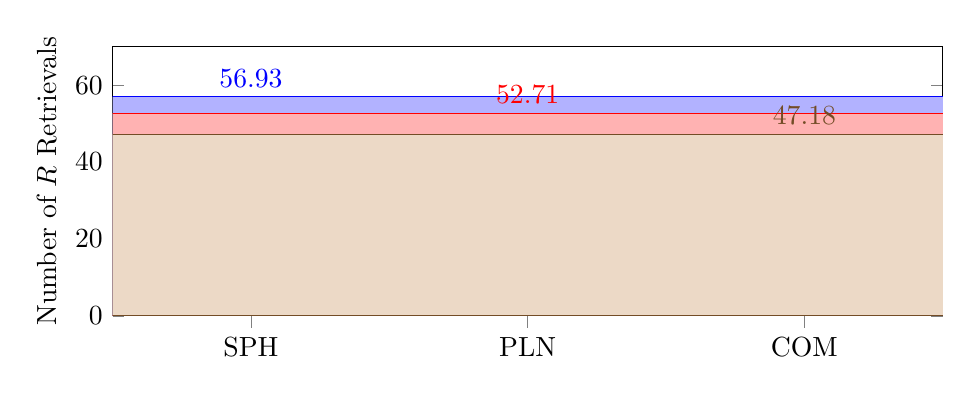
\begin{tikzpicture}
    \begin{axis}[
    ybar,
    width=\linewidth, height=5cm,
    ylabel={Number of $R$ Retrievals}, ylabel near ticks, ymin=0, ymax=70,
    xticklabels={SPH, PLN, COM},
    xtick={1, 2, 3}, xmin=0.5, xmax=3.5, xtick pos=left,
    nodes near coords, nodes near coords align={vertical},
    every axis plot/.append style={
    ybar,
    bar width=40,
    bar shift=0pt,
    fill
    }
    ]
        \addplot coordinates {(1, 56.93)}; % SPH
        \addplot coordinates {(2, 52.71)}; % PLN
        \addplot coordinates {(3, 47.18)};
    \end{axis}
\end{tikzpicture}

%SELECT AVG(QueryCount), IdentificationMethod
%FROM REDUCTION
%WHERE rowid IN (
%    SELECT rowid
%    FROM REDUCTION
%    WHERE (IdentificationMethod LIKE 'Plane' OR IdentificationMethod LIKE 'Sphere')
%    AND ShiftDeviation < 1.0e-3 AND ShiftDeviation > 1.0e-5 AND FalseStars = 0
%    AND QueryCount > 1
%)
%GROUP BY IdentificationMethod

%SELECT AVG(QueryCount)
%FROM REDUCTION
%WHERE rowid IN (
%    SELECT rowid
%    FROM REDUCTION
%    WHERE IdentificationMethod LIKE 'Composite'
%    AND ShiftDeviation < 1.0e-3 AND ShiftDeviation > 1.0e-5 AND FalseStars = 0
%    AND QueryCount > 1
%)
%    \caption{
%    Depicts the average number of database accesses required to obtain a $r$ set for strategies with triangular features given $\sigma \seq \ang{0.0001}$ of Gaussian noise.
%    To characterize the pivoting method itself, we only display instances where $\abs{R}\!\neq\!1$ with the first $b$ selection.
%%    The Spherical Triangle strategy has $1{,}952 / 2{,}000$ runs matching the criteria before, the Planar Triangle
%%    strategy has $1{,}946$ runs, and the Composite Pyramid strategy has $1{,}957$ runs.
%    }\label{fig:rPivot}
%    }
%\end{figure}

%\subsubsection{How expensive is the pivoting process?}
%import numpy as np
%m_1, m_2, s_1, s_2, n_1, n_2 = 52.71, 47.18, 56.794658219949106, 47.01765577951369, 1946, 1957
%z = (m_2 - m_1) / np.sqrt( ((s_1 * s_1) / n_1) + ((s_2 * s_2) / n_2) )
%As seen previously, identification strategies with triangular features have the most instances where $\abs{R} \seq 1$ given an image with no noise.
%~\autoref{fig:rPivot} displays the average number of database accesses for these same strategies where the first image set $b$ selection does not meet the $R$ criterion given an image with Gaussian noise.
%The average number of database accesses is higher in strategies that use the pivoting processes, as opposed to those that do not.
%Given the null hypothesis that the difference between the Planar Triangle strategy's number of database accesses and the Composite Pyramid strategy's number of database accesses is not significant, $z \seq 3.3, p\!<\!0.0001$ is obtained with a two-tailed two sample $Z$ test.
%With the data collected here, we find that the pivoting process results in more database accesses on average.
%This increased number of accesses results in a $6.70\si{ms}$ difference on average between the two.
%
%The pivoting process was only tested with the strategies most frequently meeting the $\abs{R}\seq1 $ criterion.
%An area of interest would be to see the effects of applying this process to strategies with angular features (i.e.\ Angle, Interior Angle, Pyramid).
%These strategies met the criterion less frequently, and would likely benefit from attempting to reduce the $R$ set before deciding to choose another $b$ set.
%
%\subsection{Confidence Check}\label{subsec:identificationStep}
%\subsubsection{How effective is a second confidence check?}
%if __name__ == '__main__':
%from numpy import std, average, sqrt
%from sqlite3 import connect
%from os import environ
%
%conn_1 = connect(environ['HOKU_PROJECT_PATH'] + '/data/lumberjack-all-triad.db')
%conn_2 = connect(environ['HOKU_PROJECT_PATH'] + '/data/lumberjack-pyramid-noverify.db')
%
%name = 'Pyramid'
%
%sample_1 = list(map(lambda b: b.execute("""
%SELECT PercentageCorrect
%FROM IDENTIFICATION
%WHERE ShiftDeviation < 1.0e-7 AND FalseStars = 0
%AND IdentificationMethod LIKE '{}'
%""".format(name)).fetchall(), [conn_1, conn_2]))
%
%sample_2 = list(map(lambda b: b.execute("""
%SELECT PercentageCorrect
%FROM IDENTIFICATION
%WHERE ShiftDeviation < 1.0e-5 AND FalseStars = 0
%AND IdentificationMethod LIKE '{}'
%""".format(name)).fetchall(), [conn_1, conn_2]))
%
%sample_3 = list(map(lambda b: b.execute("""
%SELECT PercentageCorrect
%FROM IDENTIFICATION
%WHERE ShiftDeviation < 1.0e-2 AND ShiftDeviation > 1.0e-4 AND FalseStars = 0
%AND IdentificationMethod LIKE '{}'
%""".format(name)).fetchall(), [conn_1, conn_2]))
%
%flatten = lambda a: [b[0] for b in a]
%for i, sample in enumerate([sample_1, sample_2, sample_3]):
%n_1, n_2 = 2000, 2000
%m_1, m_2 = average(flatten(sample[0])), average(flatten(sample[1]))
%s_1, s_2 = std(flatten(sample[0])), std(flatten(sample[1]))
%print('Z Score of {}: {}'.format(i, (m_2 - m_1) / sqrt( ((s_1 * s_1) / n_1) + ((s_2 * s_2) / n_2) )))

%import numpy as np
%print(np.average( [6.97725 - 3.00525, 6.9615 - 3.005, 398.0655 -  ))
%In~\autoref{fig:verify}, the accuracy of the map produced by the Pyramid and Composite Pyramid strategies are displayed with and without the second confidence check for varying levels of Gaussian noise.
%In~\autoref{algorithm:pyramidIdentification}, this refers to the \Call{ConfidenceCheck}{} function.
%Without noise, the Pyramid strategy without its second confidence check is 4.33\% less accurate than the Pyramid strategy with its original configuration on average.
%This behavior is consistently seen for Gaussian noise of $\sigma\seq\ang{0.000001}$ \& $\sigma\seq\ang{0.001}$, and can be attributed to the more frequent rejection of incorrect maps with $R$ sets that have met the criterion.
%In the $\sigma\seq\ang{0.001}$ case, there exists a difference of 389.95 accesses between both variations of the Pyramid and a 15\% mapping accuracy difference in favor of the strategy with the original configuration.
%Given the null hypotheses that the difference between both variations of the Pyramid strategy are different for each level of noise, $z_0 \seq 15.87, z_{0.000001} \seq 16.04, z_{0.001} \seq 12.14$ (all $p\!<\!0.0001$) is obtained with two-tailed two sample $Z$ tests.
%The verification step increases the accuracy of the Pyramid strategy.
%
%\begin{figure}
%    \centering{
%        \begin{tikzpicture}
    \begin{axis}[
    ybar,
    width=\linewidth, height=5cm,
    ylabel={$a(h, b, r)$}, ylabel near ticks, ymin=0, ymax=1.3,
    xtick={1, 2, 3}, xticklabels={$\ang{0}$, $\ang{0.000001}$, $\ang{0.001}$},
    xlabel={$\sigma$ of Noise (degrees)}, xmin=0.5, xmax=3.5, xtick pos=left,
    nodes near coords, every node near coord/.append style={rotate=90, anchor=west},
    legend style={at={(0.5,-0.35)}, anchor=north,legend columns=-1},
    bar width=7
    ]
        \addplot coordinates {(1, 0.999416666666667) (2, 0.999222222222222) (3, 0.354333333333333)};
        \addplot coordinates {(1, 0.956083333333329) (2, 0.954444444444449) (3, 0.203166666666665)};
        \addplot coordinates {(1, 1.0) (2, 1.0) (3, 0.0)};
        \addplot coordinates {(1, 1.0) (2, 0.999833333333333) (3, 0.346333333333333)};
        \legend{PYR, PYR-N, COM, COM-N}
    \end{axis}
\end{tikzpicture}
%        \caption{
%        Depicts the frequency of correct maps (\texttt{ACC}) formed with and without the second confidence step (\Call{ConfidenceCheck}{}) of both the Pyramid and Composite Pyramid strategies.
%        There exists $2{,}000$ runs for each identification strategy, with a database access limit (i.e.\ number of times the database is searched) of 500.
%        The `-N' suffix indicates the strategy bypasses \Call{ConfidenceCheck}{}.
%%        PYR corresponds to the Pyramid method with the verification step, PYR-N corresponds to the Pyramid method
%%        without the verification step, COM corresponds to the Composite Pyramid method with the verification step,
%%        and COM-N corresponds to the Composite Pyramid method without the verification step.
%        }\label{fig:verify}
%    }
%\end{figure}
%
%\begin{figure*} % HAD TO MOVE THIS GUY TOO...
%    \centering{
%    \begin{subfigure}[b]{0.48\linewidth}
%        \begin{tikzpicture}
    \begin{axis}[
    ybar,
    width=\linewidth, height=5cm,
    ylabel={$t \ (\si{ms})$}, ylabel near ticks, ymin=10, ymax=100000,
    xtick={1, 2, 3}, xticklabels={$\ang{0}$, $\ang{0.0001}$, $\ang{0.01}$},
    xlabel={$\sigma$ (degrees)}, xmin=0.5, xmax=3.5, xtick pos=left, point meta=rawy,
    nodes near coords, every node near coord/.append style={rotate=90, anchor=west,
    /pgf/number format/.cd,fixed,precision=6},
    legend style={at={(0.5,-0.35)}, anchor=north,legend columns=-1},
    bar width=7, ymode=log, log origin=infty, max space between ticks=20
    ]
        \addplot coordinates {(1, 1197.43) (2, 1349.07) (3, 6509.00)};
        \addplot coordinates {(1, 160.68) (2, 161.80) (3, 872.22)};
        \addplot coordinates {(1, 323.94) (2, 339.23) (3, 392.29)};
        \addplot coordinates {(1, 324.35) (2, 328.85) (3, 352.24)};
        \addplot coordinates {(1, 170.79) (2, 171.53) (3, 364.04)};
        \addplot coordinates {(1, 405.53) (2, 1545.45) (3, 362.30)};
        \legend{ANG, INT, SPH, PLN, PYR, COM}
    \end{axis}
\end{tikzpicture}
%    \end{subfigure}
%    \begin{subfigure}[b]{0.48\linewidth}
%        %if __name__ == '__main__':
%    from numpy import std, average, sqrt, polyfit, log
%    from sqlite3 import connect
%    from os import environ
%
%    conn_1 = connect(environ['HOKU_PROJECT_PATH'] + '/data/lumberjack-all-triad.db')
%    cur = conn_1.cursor()
%
%    # 1,   2,      3,      4,      5,     6,    7,   8
%    # 0.0, 1.0e-6, 1.0e-5, 0.0001, 0.001, 0.01, 0.1, 1.0
%
%    for d in [[1, 2, 3, 4, 5, 6, 7, 8], [0.0, 1.0e-6, 1.0e-5, 0.0001, 0.001, 0.01, 0.1, 1.0]]:
%        t = polyfit(log(d[3:]), [0.9725, 0.386, 0.0035, 0.0, 0.0], 1)
%        print('Angle: {}*ln(x) + {}'.format(t[0], t[1]))
%
%        t = polyfit(log(d[4:]), [0.9885, 0.7055, 0.033, 0.00383333333333333], 1)
%        print('Dot: {}*ln(x) + {}'.format(t[0], t[1]))
%
%        t = polyfit(log(d[2:]), [0.9715, 0.8135, 0.259, 0.0253333333333333, 0.0095, 0.00716666666666667], 1)
%        print('Sphere: {}*ln(x) + {}'.format(t[0], t[1]))
%
%        t = polyfit(log(d[2:]), [0.9865, 0.8615, 0.332166666666667, 0.0245, 0.0095, 0.00483333333333333], 1)
%        print('Plane: {}*ln(x) + {}'.format(t[0], t[1]))
%
%        t = polyfit(log(d[3:]), [0.999333333333334, 0.354333333333333, 0.0, 0.0, 0.0], 1)
%        print('Pyramid: {}*ln(x) + {}'.format(t[0], t[1]))
%
%        t = polyfit(log(d[1:]), [1.0, 0.65, 0.0035, 0.0, 0.0, 0.0, 0.0], 1)
%        print('Composite: {}*ln(x) + {}'.format(t[0], t[1])), print()

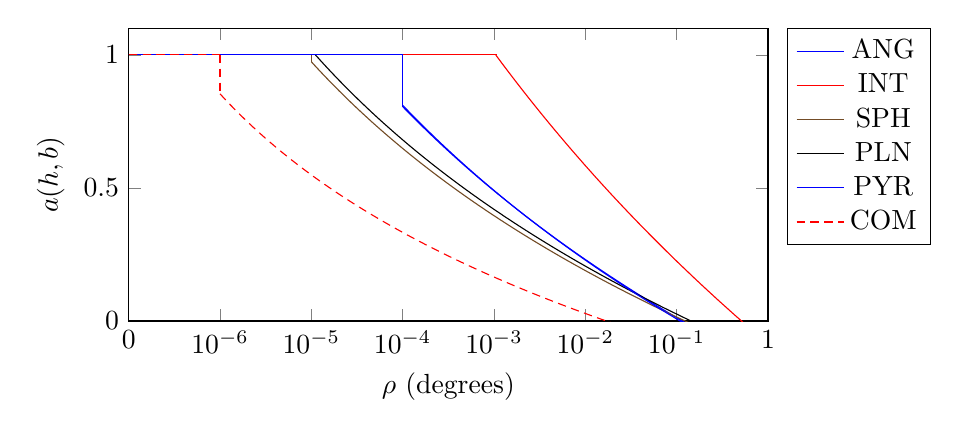
\begin{tikzpicture}
    \begin{axis}[
    width=0.8\linewidth, height=5.3cm,
    ylabel={$a(h, b)$}, ymin=0, ymax=1.1,
    xlabel={$\rho$ (degrees)}, xmin=1, xmax=8,
    xtick={1, 2, 3, 4, 5, 6, 7, 8},
    xticklabels={$0$, $10^{-6}$, $10^{-5}$, $10^{-4}$, $10^{-3}$, $10^{-2}$, $10^{-1}$, $1$},
    samples=100, no markers, legend pos=outer north east, enlargelimits=false
    ]
        \addplot +[domain=1:4, forget plot]{1};
        \addplot +[forget plot] coordinates {(4, 1) (4, 0.8055384229041530)};
        \addplot +[domain=4:8]{-1.416887591459587*ln(x) + 2.7697617012853217};
        \addlegendentry{ANG}

        \addplot +[domain=1:5.03, forget plot]{1};
%        \addplot +[forget plot] coordinates {(5, 1) (5, 1)};
        \addplot +[domain=5.02:8]{-2.3292306442173216*ln(x) + 4.757244753386215};
        \addlegendentry{INT}

        \addplot +[domain=1:3, forget plot]{1};
        \addplot +[forget plot] coordinates {(3, 1) (3, 0.9738787471803161)};
        \addplot +[domain=3:8]{-1.1317828984553227*ln(x) + 2.217269347527745};
        \addlegendentry{SPH}

        \addplot +[domain=1:3, forget plot]{1};
%        \addplot +[forget plot] coordinates {(3, 1) (3, )};
        \addplot +[domain=3.04:8]{-1.1696544292494204*ln(x) + 2.301996347627258};
        \addlegendentry{PLN}

        \addplot +[domain=1:4, forget plot]{1};
        \addplot +[forget plot] coordinates {(4, 1) (4, 0.8105837347641904)};
        \addplot +[domain=4:8]{-1.4347255837709008*ln(x) + 2.7995357213002334};
        \addlegendentry{PYR}

        \addplot +[domain=1:2, forget plot]{1};
        \addplot +[forget plot] coordinates {(2, 1) (2, 0.8533960244900531)};
        \addplot +[domain=2:8]{-0.7510156659772902*ln(x) + 1.3739604159185614};
        \addlegendentry{COM}
    \end{axis}
\end{tikzpicture}
%    \end{subfigure}
%    \caption{
%    Both plots represent a statistic about the resulting map $h$ produced by each identification strategy given some image with varying Gaussian noise.
%    There exists $2{,}000$ runs for each identification strategy, with the number of database accesses limited to 500.
%    The left plot depicts the average time to obtain $h$, and the right plot depicts the trend line $\texttt{ACC} = c \cdot \mathit{\ln}\left( \sigma \right) + d$.
%    }\label{fig:gaussianNoise}
%    }
%\end{figure*}

%The response to Gaussian noise for the Composite Pyramid begins at $\sigma\seq\ang{0.001}$, with a 34.6\% difference between the two variants in favor of the strategy without the second confidence check.
%Unlike the second confidence check in the Pyramid strategy, this filter appears to be too aggressive for the Composite Pyramid strategy.
%The variant without the second confidence check has an average of 193.93 database accesses at $\sigma\seq\ang{0.001}$.
%Without the second confidence check, the Composite Pyramid strategy only had an average of 8.114 database accesses, suggesting that the $\abs{R} \seq 1$ criterion and the \Call{DMT}{} process are sufficient enough for rejecting incorrect $R$ sets and maps.
%
%\subsection{End to End}\label{subsec:endToEndEvaluation}
%\subsubsection{Which strategy is the fastest given no noise?}
%In~\autoref{fig:gaussianNoise}, the left plot depicts the end to end running time of each identification strategy given varying degrees of Gaussian noise.
%In the no noise case, the Angle strategy is the slowest identification strategy on average.
%The next slowest strategy is the Composite Pyramid strategy, a factor of 2.95 times faster than the Angle strategy.
%Recall that the Angle strategy had the fastest candidate retrieval, but the largest $\abs{R}$.
%On average, it takes 69.85 database accesses to obtain a mapping and 68.10 database accesses to meet the $\abs{R} \seq 1$ criterion.
%This suggests that the Angle strategy's long running time stems from the $\abs{R} \seq 1$ criterion and not the \Call{DMT}{} process.

%import numpy as np
%m_1, m_2, s_1, s_2, n_1, n_2 = 160.675, 170.7905, 0.53808, 0.52922, 2000, 2000
%z = (m_2 - m_1) / np.sqrt( ((s_1 * s_1) / n_1) + ((s_2 * s_2) / n_2) )
%The fastest strategy in the no noise case appears to be the Interior Angle strategy, with the second fastest strategy running 10.11 \si{ms} slower.
%There exists $0 / 2{,}000$ runs where the Interior Angle strategy runs above the Pyramid strategy's average running time ($170.79$ $\si{ms}$) and the Interior Angle strategy has the fastest recorded identification run of $135\si{ms}$.
%The Interior Angle strategy is the fastest identification strategy given no noise.

%\subsubsection{Which strategy is the fastest given varying levels of Gaussian noise?}
%As Gaussian noise is increased from $\sigma\seq\ang{0}$ to $\sigma\seq\ang{0.01}$, the Angle strategy experiences the largest response of $5{,}311.57$ additional $\si{ms}$.
%The next slowest strategy in the noise of $\rho\seq\ang{0.01}$ case is the Interior Angle strategy, a factor of 7.46 times faster than the Angle strategy.
%On average, the Angle strategy takes 399.66 database accesses to obtain a mapping and only 36.72 accesses to obtain $r$ here.
%In the no noise case, this strategy's long running time can attributed to the aggressive $R$ criterion.
%Given Gaussian noise, the \Call{DMT}{} process plays a larger role with the Angle strategy and returns to $b$ decision process more often.
%
%The Composite Pyramid strategy shows an interesting runtime response to this type of noise, running $1{,}139.92\si{ms}$ longer given $\ang{0.0001}$ of noise from no noise but $1{,}183.15\si{ms}$ shorter from $\ang{0.0001}$ of noise to $\ang{0.01}$.
%The Pyramid strategy is observed to have this same running time response against noise at $\sigma\seq\ang{0.001}$ (not depicted).
%The most probable explanation lies in how far each run travels from the $b$ decision step.
%At $\sigma\seq\ang{0.0001}$, the Composite Pyramid has gone through the $\abs{R} \seq 1$ criterion and is likely choosing another $b$ set after the verification step.
%At $\sigma\seq\ang{0.01}$ the strategy is not passing the same criterion, avoiding the verification step.

%if __name__ == '__main__':
%from numpy import std, average, sqrt
%from sqlite3 import connect
%from os import environ
%
%conn_1 = connect(environ['HOKU_PROJECT_PATH'] + '/data/lumberjack-all-triad.db')
%conn_2 = connect(environ['HOKU_PROJECT_PATH'] + '/data/lumberjack-pyramid-noverify.db')
%
%sample_1 = conn_1.execute("""
%SELECT TimeToResult
%FROM IDENTIFICATION
%WHERE ShiftDeviation > 1.0e-7 AND FalseStars = 0
%AND IdentificationMethod LIKE 'Plane'
%""").fetchall()
%
%sample_2 = conn_1.execute("""
%SELECT TimeToResult
%FROM IDENTIFICATION
%WHERE ShiftDeviation > 1.0e-7 AND FalseStars = 0
%AND IdentificationMethod LIKE 'Pyramid'
%""").fetchall()
%
%flatten = lambda a: [b[0] for b in a]
%n_1, n_2 = 12000, 12000
%m_1, m_2 = average(flatten(sample_1)), average(flatten(sample_2))
%s_1, s_2 = std(flatten(sample_1)), std(flatten(sample_2))
%print('Z Score of: {}'.format((m_2 - m_1) / sqrt( ((s_1 * s_1) / n_1) + ((s_2 * s_2) / n_2) )))
%The fastest strategy on average given images with Gaussian noise $\sigma \in \set{10^{-1}, 10^{-2}, \ldots, 10^{-6}}$ is the Pyramid strategy at $288.44$ $\si{ms}$ (of 12,000 runs).
%%\begin{equation}\label{eq:sigmasTested}
%%    \rho \in \set{10^{-1}, 10^{-2}, \ldots, 10^{-6}}
%%\end{equation}
%The second fastest strategy given the same noise set is the Planar Triangle strategy at $341.16\si{ms}$.
%Given the null hypothesis that the difference between both averages is not significant, $z \seq 24.32, p\!<\!0.0001$ is found with a two-tailed two sample $Z$ test.
%With the data collected here, the Pyramid strategy is the fastest strategy given varying amounts of Gaussian noise.
%
%\begin{figure*}
%    \centering{
%    \begin{subfigure}[b]{0.48\linewidth}
%        \begin{tikzpicture}
    \begin{axis}[
    ybar,
    width=\linewidth, height=5cm,
    ylabel={$t \ (\si{ms})$}, ylabel near ticks, ymin=10, ymax=100000,
    xtick={1, 2, 3}, xticklabels={0, 6, 12},
    xlabel={$\omega$}, xmin=0.5, xmax=3.5, xtick pos=left, point meta=rawy,
    nodes near coords, every node near coord/.append style={rotate=90, anchor=west,
    /pgf/number format/.cd,fixed,precision=2},
    legend style={at={(0.5,-0.35)}, anchor=north,legend columns=-1},
    bar width=7, ymode=log, log origin=infty, max space between ticks=20
    ]
        \addplot coordinates {(1, 1197.43) (2, 1737.94) (3, 2431.58)};
        \addplot coordinates {(1, 160.68) (2, 209.36) (3, 280.54)};
        \addplot coordinates {(1, 323.94) (2, 355.54) (3, 386.20)};
        \addplot coordinates {(1, 324.35) (2, 350.60) (3, 390.41)};
        \addplot coordinates {(1, 170.79) (2, 183.71) (3, 195.53)};
        \addplot coordinates {(1, 405.53) (2, 685.07) (3, 972.04)};
        \legend{ANG, DOT, SPH, PLN, PYR, COM}
    \end{axis}
\end{tikzpicture}
%    \end{subfigure}
%    \begin{subfigure}[b]{0.48\linewidth}
%        \begin{tikzpicture}
    \begin{axis}[
    ybar,
    width=\linewidth, height=5cm,
    ylabel={Accuracy of Map, \texttt{ACC}}, ylabel near ticks, ymin=0, ymax=1.4,
    xtick={1, 2, 3}, xticklabels={0, 6, 12},
    xlabel={$\omega$}, xmin=0.5, xmax=3.5, xtick pos=left,
    nodes near coords, every node near coord/.append style={rotate=90, anchor=west,
    /pgf/number format/.cd,fixed,precision=4},
    legend style={at={(0.5,-0.35)}, anchor=north,legend columns=-1},
    bar width=7
    ]
        \addplot coordinates {(1, 0.977) (2, 0.979) (3, 0.960)};
        \addplot coordinates {(1, 1.0) (2, 0.982) (3, 0.965)};
        \addplot coordinates {(1, 1.0) (2, 0.840) (3, 0.696)};
        \addplot coordinates {(1, 1.0) (2, 0.845) (3, 0.703)};
        \addplot coordinates {(1, 0.999) (2, 0.999) (3, 0.995)};
        \addplot coordinates {(1, 1.0) (2, 0.994) (3, 0.973)};
        \legend{ANG, INT, SPH, PLN, PYR, COM}
    \end{axis}
\end{tikzpicture}
%    \end{subfigure}
%    \caption{
%    Both plots represent a statistic about the resulting map $h$ produced by each identification strategy given some image with varying amounts of spikes $\omega$.
%    There exists $2{,}000$ runs for each identification strategy, with the number of database accesses limited to 500.
%    The left plot depicts the average time to obtain a map $h$, and the right plot depicts the average accuracy of the produced $h$.
%    }\label{fig:falseNoise}
%    }
%\end{figure*}

%\subsubsection{Which strategy has the slowest growing map accuracy response to increasing noise?}
%The selection of the retrieval $\epsilon$ parameters plays a significant role in accuracy of each strategy given images with Gaussian noise.
%For strategies that search the database using on the $\theta$ feature (Angle, Interior Angle, Pyramid), the $\epsilon$ parameter serves as a rough upper bound for the amount of Gaussian noise tolerated.
%In~\autoref{fig:gaussianNoise}, the plot on the right depicts the accuracy of resulting injection of each method for
%varying levels of Gaussian noise.
%When the level of noise is equal to the Angle and Pyramid $\epsilon_\theta$ parameter ($\ang{0.0001}$), both strategies have an average $h$ accuracy of $98.59\!\pm\!1.34\%$.
%When Gaussian noise is increased to $\ang{0.001}$, both strategies drop to $47.02\!\pm\!1.58\%$.

%For strategies with features that are not angular (Spherical Triangle, Planar Triangle, Composite Pyramid), characterizing the effect of Gaussian noise becomes more difficult.
%These strategies have the parameters $\epsilon_a \seq 3\cdot 10^{-9}$ and $\epsilon_\tau \seq 3\cdot10^{-9}$, showing an initial accuracy response to noise at $\ang{0.00001}$.
%The Interior Angle method has the largest query $\sigma$ parameters, and only experiences a response to noise at
%$\ang{0.01}$.
%Given the current set of query $\sigma$, the Interior Angle is the most accurate method on average.

%Ranking each strategy based on their $h$ accuracy is not particularly insightful here given the heavy dependence on $\epsilon$ parameters, so instead we analyze the rate of change involved with varying levels of noise.
%The right plot in~\autoref{fig:gaussianNoise} depicts the trend line for all strategies where $h$ accuracy (denoted as \texttt{ACC}) is displayed against the amount of Gaussian noise.
%It has been observed that the accuracy of each strategy remains near 100\% until it decreases exponentially to zero:
%\begin{equation}
%    \texttt{ACC} =
%    \begin{cases}
%        0 & \sigma < 0 \\
%        1 & 0 \leq \sigma < \hat{\sigma} \\
%        c \cdot \ln(\sigma) + d & \sigma \geq \hat{\sigma}
%    \end{cases}
%\end{equation}
%Each line was fit to the piecewise equation above ($c\cdot \ln(\sigma) + d$ term with least squares), where $c$ and $d$ are the parameters found with the regression, $\texttt{ACC}$ is the accuracy of the map $h$, and $\hat{\sigma}$ is the point where $\texttt{ACC}$ is observed to dip below 95\%.
%The accuracy acceleration varies across strategies through the value of $c$:
%\begin{equation}
%    \frac{d^{2}\texttt{ACC}}{d\sigma^2} = \frac{-c}{\sigma^2}, \ \ \sigma \geq \hat{\sigma}
%\end{equation}
%A larger $c$ suggests that a change in retrieval $\epsilon$ or Gaussian noise will not affect the accuracy of the strategy as much as a strategy with a larger $c$.
%The strategy with the largest acceleration toward $0\%$ \texttt{ACC} is the Interior Angle strategy ($c \seq -0.15749$).
%The Spherical Triangle strategy has the slowest growing \texttt{ACC} response to increasing noise ($c \seq -0.09266$).
%
%\subsubsection{Which strategy is the fastest given varying amounts of false points?}
%In~\autoref{fig:falseNoise}, the plot on the left depicts the end to end running time of each strategy given varying amounts of spikes (i.e.\ false points).
%As the number of spikes increases from 0 to 12, the Angle strategy again experiences the largest response of $1{,}234.15$ $\si{ms}$.
%The next fastest strategy is the Composite Pyramid strategy, a factor of 2.50 times faster than the Angle strategy.
%The difference between the 1st and 2nd slowest strategies is 2.98 times less than the Gaussian noise case.
%On average, it takes 114.23 database accesses to obtain a map and only 54.85 accesses to obtain $r$.
%Relative to the Gaussian noise comparison, \Call{DMT}{} and $\abs{R} \seq 1$ criterion play a more equal role in the decision to choose a new $b$ set.

%if __name__ == '__main__':
%from numpy import std, average, sqrt
%from sqlite3 import connect
%from os import environ
%
%conn_1 = connect(environ['HOKU_PROJECT_PATH'] + '/data/lumberjack-all-triad.db')
%conn_2 = connect(environ['HOKU_PROJECT_PATH'] + '/data/lumberjack-pyramid-noverify.db')
%
%sample_1 = conn_1.execute("""
%SELECT TimeToResult
%FROM IDENTIFICATION
%WHERE FalseStars > 0
%AND IdentificationMethod LIKE 'Pyramid'
%""").fetchall()
%
%sample_2 = conn_1.execute("""
%SELECT TimeToResult
%FROM IDENTIFICATION
%WHERE FalseStars > 0
%AND IdentificationMethod LIKE 'Dot'
%""").fetchall()
%
%flatten = lambda a: [b[0] for b in a]
%n_1, n_2 = 8000, 8000
%m_1, m_2 = average(flatten(sample_1)), average(flatten(sample_2))
%s_1, s_2 = std(flatten(sample_1)), std(flatten(sample_2))
%print('Z Score of: {}'.format((m_2 - m_1) / sqrt( ((s_1 * s_1) / n_1) + ((s_2 * s_2) / n_2) )))
%The fastest strategy on average given images with spikes is the Pyramid strategy at $186.22\si{ms}$.
%The images given to each strategy contained $\omega$ spikes, where $\omega \in \set{ 3, 6, 9, 12 }$.
%The second fastest strategy given the same noise set is the Interior Angle strategy at $228.37\si{ms}$.
%Given the null hypothesis that the difference between both averages is not significant, $z \seq 28.47, p\!<\!0.0001$ is
%found with a two-tailed two sample $Z$ test.
%The Pyramid strategy is the fastest strategy given varying amounts of spikes.
%The process for choosing distinct image subsets is shown to be the fastest approach to finding a map that meets the Pyramid's confidence checks.

%if __name__ == '__main__':
%from numpy import std, average, sqrt, polyfit, log
%from sqlite3 import connect
%from os import environ
%
%conn_1 = connect(environ['HOKU_PROJECT_PATH'] + '/data/lumberjack-all-triad.db')
%cur = conn_1.cursor()
%
%for name in ['Angle', 'Dot', 'Sphere', 'Plane', 'Pyramid', 'Composite']:
%sample_1 = list(map(lambda a: a[0], cur.execute("""
%SELECT AVG(TimeToResult)
%FROM IDENTIFICATION
%WHERE FalseStars > 0
%AND IdentificationMethod LIKE ?
%GROUP BY FalseStars
%ORDER BY FalseStars
%""", (name, )).fetchall()))
%
%t = polyfit([3, 6, 9, 12], sample_1, 1)
%print('{name}: {t_0}*x + {t_1}'.format(name=name, t_0=round(t[0], 5), t_1=round(t[1], 5)))
%Each strategy exhibits a linear increase to runtime as additional spikes are added.
%To characterize each strategy's runtime as a function of false points, each strategy's runtime was fit to a linear equation using least squares:
%\begin{equation}
%    t = c\cdot\omega + d
%\end{equation}
%where $c$ and $d$ are the parameters found with the regression and $t$ is the end to end running time of the strategy.
%A smaller $\abs{c}$ suggests that the number of spikes will affect the end to end runtime than that of a strategy with a larger $\abs{c}$.
%The strategy with the largest $\abs{c}$ is the Angle strategy with $c \seq -414.559$.
%The strategy with the smallest $\abs{c}$ term is the Pyramid strategy with $c \seq -6.766$.
%The Pyramid strategy is the fastest given varying amounts of false points, having a runtime that is also the least responsive to increasing spikes.

%\subsubsection{Which strategy is the most accurate given varying amounts of false points?}
%if __name__ == '__main__':
%from numpy import std, average, sqrt
%from sqlite3 import connect
%from os import environ
%
%conn_1 = connect(environ['HOKU_PROJECT_PATH'] + '/data/lumberjack-all-triad.db')
%conn_2 = connect(environ['HOKU_PROJECT_PATH'] + '/data/lumberjack-pyramid-noverify.db')
%
%sample_1 = conn_1.execute("""
%SELECT PercentageCorrect
%FROM IDENTIFICATION
%WHERE FalseStars = 12
%AND (IdentificationMethod LIKE 'Plane' OR IdentificationMethod LIKE 'Sphere')
%""").fetchall()
%
%sample_2 = conn_1.execute("""
%SELECT PercentageCorrect
%FROM REDUCTION
%WHERE FalseStars = 12
%AND (IdentificationMethod LIKE 'Plane' OR IdentificationMethod LIKE 'Sphere')
%""").fetchall()
%
%flatten = lambda a: [b[0] for b in a]
%n_1, n_2 = 2000, 2000
%m_1, m_2 = average(flatten(sample_1)), average(flatten(sample_2))
%s_1, s_2 = std(flatten(sample_1)), std(flatten(sample_2))
%print('Z Score of: {}'.format((m_2 - m_1) / sqrt( ((s_1 * s_1) / n_1) + ((s_2 * s_2) / n_2) )))
%In~\autoref{fig:falseNoise}, the plot on the right depicts the average accuracy of each mapping given varying amounts of spikes.
%As the number of false points is increased from $\omega \seq 0$ to $\omega \seq 12$, the strategies that experience the largest $h$ accuracy response are the Spherical Triangle strategy ($30.42\%$ average decrease) and the Planar Triangle strategy ($29.68\%$ average decrease).
%The average accuracy of the candidate selection is a few percent less than the average accuracy of $h$ here ($0.53\!\pm\!1.78\%$ for both strategies).
%Given the null hypothesis that the difference between the accuracy of the $h$ map and the accuracy of the candidate selection is not significant, $z \seq 0.37, p \seq 0.71$ was found with a two-tailed two sample $Z$ test.
%There does not exist enough data to reject this hypothesis with $\alpha \seq 0.01$.
%This suggests that the \Call{DMT}{} process is neither helpful or detrimental to the end to end accuracy of these strategies.
%
%Ruling out the \Call{DMT}{} process, the most likely source of error for the triangle strategies is their decision of different $b$ sets.
%If a false point exists as $b[1]$ in $b$, the triangle strategies will have to iterate through $n^2$ combinations and $n - 3$ pivots at most to choose another point that is not the spike.
%The Angle strategy only has to wait $n$ additional combinations at most if a false point exists in $b$.
%The Interior Angle strategy is able to get around the spike persistence problem by choosing $b$ sets based on their $\theta$ proximity to the central point.
%The Pyramid and Composite Pyramid strategies have their $b$ decision process designed for this situation, increasing the average turnover of all points in the $b$ set.
%
%The Pyramid strategy has the most accurate map $h$ on average given images with all different $\omega$ at $99.84\!\pm\!3.53\%$.
%The second most accurate strategy is the Composite Pyramid strategy at $99.19\!\pm\!8.95\%$.
%Given the null hypothesis that the difference between the mapping accuracies of both strategies is not significant, $z \seq 3.02, p \seq 0.003$ with a two-tailed two sample $Z$ test.
%At $\alpha \seq 0.01$, our hypothesis does not hold true.
%The Pyramid strategy is the most accurate under varying amounts of spikes.

%	\input{include/conclusion-shr}
    %\section{Acknowledgements}\label{sec:acknowledgements}
\begin{acks}
	We would like to thank Dr. Miguel Nunes, Eric Pilger, and Yosef Ben Gershom from the Hawaii Space Flight Laboratory for providing input toward the creation of software for a first generation star tracker.
\end{acks}
    \balance

%	\nocite{*}
	\bibliographystyle{ACM-Reference-Format}
	\bibliography{include/references}

\end{document}
